\documentclass[12pt]{article}
%\topmargin=-0.5in
%\textheight=9in
%\evensidemargin=0in
%\oddsidemargin=0in
%\setlength{\textwidth}{6.5in}

\usepackage{amsmath,latexsym}
\usepackage{amsfonts}
\usepackage{amssymb}
\usepackage{amssymb}
\usepackage{caption}
\usepackage{graphicx}
%\usepackage{appendix}
%\usepackage{clrscode3e}
\usepackage{epstopdf}
\usepackage{subfigure}
%\usepackage{algorithm}
%\usepackage{algorithmic}
\usepackage{setspace}
\usepackage{color}
\usepackage{listings}
\usepackage{setspace}
\usepackage{algpseudocode}
\usepackage{algorithm}
\usepackage[all]{xy}
\usepackage{pdfpages}

% Glossary stuff - put definitions in defns.tex file
\usepackage{glossaries}
\loadglsentries{definitions}
\makenoidxglossaries

% double spacing!
\doublespacing

\renewcommand{\topfraction}{0.9}	% max fraction of floats at top
\renewcommand{\bottomfraction}{0.8}	% max fraction of floats at bottom
%   Parameters for TEXT pages (not float pages):
\setcounter{topnumber}{2}
\setcounter{bottomnumber}{2}
\setcounter{totalnumber}{4}      % 2 may work better
\setcounter{dbltopnumber}{2}    % for 2-column pages
\renewcommand{\dbltopfraction}{0.9}	% fit big float above 2-col. text
\renewcommand{\textfraction}{0.07}	% allow minimal text w. figs
%   Parameters for FLOAT pages (not text pages):
    \renewcommand{\floatpagefraction}{0.7}	% require fuller float pages
% N.B.: floatpagefraction MUST be less than topfraction !!
\renewcommand{\dblfloatpagefraction}{0.7}	% require fuller float pages

% turn off all hyphenation
%\hyphenpenalty 10000
%\exhyphenpenalty 10000

% setup some colors for the code listing
\definecolor{codegreen}{rgb}{0,0.6,0}
\definecolor{codegray}{rgb}{0.5,0.5,0.5}
\definecolor{codepurple}{rgb}{0.58,0,0.82}
\definecolor{backcolour}{rgb}{0.95,0.95,0.92}
\lstdefinestyle{mystyle}{
    backgroundcolor=\color{backcolour},   
    commentstyle=\color{codegreen},
    keywordstyle=\color{magenta},
    numberstyle=\tiny\color{codegray},
    stringstyle=\color{codepurple},
    basicstyle=\tiny,
    breakatwhitespace=false,         
    breaklines=true,                 
    captionpos=b,                    
    keepspaces=true,                 
    numbers=left,                    
    numbersep=5pt,                  
    showspaces=false,                
    showstringspaces=false,
    showtabs=false,                  
    tabsize=2
}
\lstset{style=mystyle}

\newenvironment{dig}{\\ [6pt]\noindent {\bf Digression}}{~$\Box$\\ [6pt]\indent}
\newenvironment{dig1}{\noindent {\bf Digression}}{~$\Box$\\ [6pt]\indent}
\newtheorem{alg}{\hspace{1.3in} Algorithm}
\newtheorem{thrm}{Theorem}
\newtheorem{lemm}[thrm]{Lemma}
\newtheorem{conj}[thrm]{Conjecture}
%\newtheorem{claim}[thrm]{Claim}
\newtheorem{prop}[thrm]{Proposition}
\newtheorem{defn}[thrm]{Definition}
\newtheorem{obs}[thrm]{Observation}

\hyphenation{Chris-to-dou-lak-is}
\def\proof{\bigbreak\noindent {\sl Proof.\/}\enspace}
\def\qedbox#1#2{\vbox{\hrule height.2pt
  \hbox{\vrule width.2pt height#2pt \kern#1pt \vrule width.2pt}
  \hrule height.2pt}}
\def\qed{\hfill \quad\qedbox46\newline\smallbreak}

\def\s#1{\mbox{\boldmath $#1$}}
\def\floor#1{\lfloor #1 \rfloor}
\def\bfloor#1{\big\lfloor #1 \big\rfloor}
\def\Bfloor#1{\Big\lfloor #1 \Big\rfloor}
\def\ceil#1{\lceil #1 \rceil}
\def\bceil#1{\big\lceil #1 \big\rceil}
\def\+{\!+\!}
\def\-{\!-\!}
\def\plmi{\!\pm\!}
\def\m{\!-\!}
\def\uu#1{\underline{#1}}
\def\o#1{\overline{#1}}
\def\itbf#1{\textit{\textbf{#1}}}
\def\match{\approx}
\def\cP{\mathcal{P}}
\def\G{\mathcal{G}}
\def\B{\mathcal{B}}
\def\O{\mathcal{O}}

\def\bproc{{\bf procedure\ }}
\def\bfunc{{\bf function\ }}
\def\bvar{{\bf var\ }}
\def\barray{{\bf array\ }}
\def\bof{{\bf of\ }}
\def\bfor{{\bf for\ }}
\def\bnull{{\bf null\ }}
\def\bto{{\bf to\ }}
\def\bdownto{{\bf downto\ }}
\def\bwhile{{\bf while\ }}
\def\brep{{\bf repeat\ }}
\def\buntil{{\bf until\ }}
\def\band{{\bf and\ }}
\def\bor{{\bf or\ }}
\def\bdo{{\bf do\ }}
\def\bif{{\bf if\ }}
\def\bthen{{\bf then\ }}
\def\belse{{\bf else\ }}
\def\belsif{{\bf elsif\ }}
\def\bnot{{\bf not\ }}
\def\bgoto{{\bf goto\ }}
\def\bcontinue{{\bf continue\ }}
\def\breturn{{\bf return\ }}
\def\bbreak{{\bf break\ }}
\def\boutput{{\bf output}}
\def\la{\leftarrow}
\def\ra{\rightarrow}
\def\llra{\Leftrightarrow}
\def\q{\quad}
\def\qq{\qquad}
\def\com#1{{\bf $\triangleright$}\hspace{6pt}{\sl #1}}
\def\rem#1{\hspace{24pt}{\sl #1}}
\def\pref(#1,#2){$#1$ is a prefix of $#2$}
\def\suff(#1,#2){$#1$ is a suffix of $#2$}
\def\FIND{\mbox{FIND}}
\def\reg(#1,#2){$#2$ is $#1$-regular}
\def\notreg(#1,#2){$#2$ is not $#1$-regular}
\def\top{\tt{top}}
\def\pop{\tt{pop}}
\def\push{\tt{push}}
\def\true{\tt{true}}
\def\false{\tt{false}}
\def\UPDATE\_F{\tt{UPDATE\_F}}
\def\LEAST{\tt{LEAST}}
\def\MERGE{\tt{MERGE}}
\def\mec{\tt{mec}}
\def\MEC{\tt{MEC}}
\def\CMEC{\tt{CMEC}}
\def\MELC{\tt{MELC}}
\def\CMELC{\tt{CMELC}}
\def\MELS{\tt{MELS}}
\def\CMELS{\tt{CMELS}}
\def\MCNT{\tt{MaxCount}}
\def\CLEN{\tt{CorLen}}

% \def\B{\tt{B}}
\def\Q'{\tt{Q'}}
\def\CP{\tt{CP}}
\def\MNC{\tt{MNC}}
\def\PR{\tt{PR}}
\def\PRS{\tt{PRS}}
\def\CPR{\tt{CPR}}
% \def\POS{\tt{POS}}
\def\LEN{\tt{LEN}}
\newcommand{\dd}{\mathinner{\ldotp\ldotp}}

% verbatim single quote fixer
\makeatletter
\let \@sverbatim \@verbatim
\def \@verbatim {\@sverbatim \verbatimplus}
{\catcode`'=13 \gdef \verbatimplus{\catcode`'=13 \chardef '=13 }} 
\makeatother


\newif\ifShow
\Showfalse
% MATH -----------------------------------------------------------
\newcommand{\norm}[1]{\left\Vert#1\right\Vert}
\newcommand{\abs}[1]{\left\vert#1\right\vert}
\newcommand{\set}[1]{\left\{#1\right\}}
\newcommand{\Real}{\mathbb R}
\newcommand{\eps}{\varepsilon}
\newcommand{\To}{\longrightarrow}
\newcommand{\BX}{\mathbf{B}(X)}
\newcommand{\A}{\mathcal{A}}
% Algorithm ------------------------------------------------------

\algnewcommand{\LineComment}[1]{\State \(\triangleright\) \normalfont{\sl #1}}
\algtext*{EndWhile}% l
\algtext*{EndIf}% Remove "end if" text
\algtext*{EndFor}% Remove "end for" text
\algtext*{EndFor}% Remove "end for" text
\algtext*{EndProcedure}% Remove "end procedure" text

% manifold
\newcommand{\F}{{F}}
\newcommand{\scF}{\F}
\newcommand{\X}{{X}}
\newcommand{\Fhat}{\widehat\F}
\newcommand{\scN}{{\EuScript N}}
\newcommand{\scL}{{\EuScript L}}
\newcommand{\PP}{\mathbb P}
\newcommand{\R}{\mathbb R}
\newcommand{\C}{\mathbb C}
% \newcommand{\CP}{\C\PP}
\newcommand{\CH}{\C{\mathrm H}}
\newcommand{\Lie}{{\mathcal L}}
\newcommand{\cpn} {\CP^n}
\newcommand{\chn} {\CH^n}
\newcommand{\cptwo} {\CP^2}
\newcommand{\chtwo} {\CH^2}
\newcommand{\chone} {\CH^1}
%\newcommand{\mean}{{\mathcal m}}
\newcommand{\mean}{{\mathbf m}}
%\def\({\left (}
\def\({\left(}
%\def\){\right )}
\def\){\right)}
\def\<{\langle}
\def\>{\rangle}
\def\a {\alpha}
\def\b {\beta}
\def\l {\lambda}

% Pfaffian systems
\newcommand{\CC}{{\EuScript C}}
\newcommand{\I}{{\mathcal I}}
\newcommand{\J}{{\EuScript J}}
\newcommand{\K}{{\mathcal K}}
\newcommand{\Khat}{\widehat{\K}}
\newcommand{\M}{{\mathcal M}}
\newcommand{\V}{\mathcal V}
\newcommand{\calS}{\mathcal S}

% differential forms
\newcommand{\w}{\omega}
\newcommand{\kh}{\hat\kappa}
\newcommand{\diff}{{\operatorname{diff}}}
% \newcommand{\alg}{{\operatorname{alg}}}

%maps
\newcommand{\fhat}{\hat{f}}

%open sets
\newcommand{\setU}{\EuScript U}
\newcommand{\Uhat}{\widehat{\setU}}

% vectors
\newcommand{\e}{\mathbf e}
\newcommand{\ehat}{\hat{\e}}
\newcommand{\bv}{\mathbf v}
\newcommand{\bx}{\mathbf x}
\newcommand{\bg}{\mathbf g}
\newcommand{\by}{\mathbf y}
\newcommand{\bw}{\mathbf w}
\newcommand{\bxi}{\mathbf\xi}
\newcommand{\bn}{\mathbf n}
\newcommand{\bz}{\mathbf z}

% complex variables
\newcommand{\ri}{\mathrm i}
\newcommand{\realpart}{\operatorname{Re}}

% operators
\newcommand{\JJ}{{\mathrm J}} % complex structure
\newcommand{\RR}{{\sf R}} % curvature operator
\newcommand{\Ric}{{\sf Ric}} % Ricci tensor
\newcommand{\di}{\partial}
\newcommand{\dib}[1]{\di_{#1}}
\newcommand{\tvec}{\tfrac{\di}{\di t}}
\newcommand{\restr}{\negthickspace \mid}
\newcommand{\transpose}[1]{{}^t\hskip-2pt{#1}}
\newcommand{\nat}{\widetilde\nabla}
\newcommand{\RRt}{\widetilde R}
\newcommand{\mt}{\widetilde M}
\def\intprod{\mathbin{\raisebox{.4ex}{\hbox{\vrule height .5pt width
5pt depth 0pt %
         \vrule height 3pt width .5pt depth 0pt}}}}
\newcommand{\hook}{\intprod}
\def\&{\wedge}
% \def\s{\sigma}
\def\a{\alpha}
\def\b{\beta}
\def\n{\nabla}

\begin{document}

\begin{titlepage}
\pagenumbering{gobble}
\begin{center}
{\Large \bfseries SEAKER:\protect\\A Mobile Digital Forensic Triage Device \par}

\vspace{2 cm}
\baselineskip = 2\baselineskip
A Thesis Presented to \\
The Faculty of the Computer Science Department\\
California State University Channel Islands

\vspace{1 cm}

In (Partial) Fulfillment\\
of the Requirements for the Degree\\
Masters of Science in Computer Science\\

\vspace{1 cm }

\vfill

by \\
Eric Elwood Gentry\\
Advisor: Michael Soltys\\
December 2018
\end{center}
\end{titlepage}
\baselineskip = \baselineskip

\newpage
\null
\vfill
\begin{flushleft}
\copyright\; 2018\\
Eric Elwood Gentry\\
ALL RIGHTS RESERVED
\end{flushleft}
\newpage

\begin{center}
{\large \bfseries APPROVED FOR MS IN COMPUTER SCIENCE \par}

\vspace{1.5 cm}

\hrulefill\\
{\large \bfseries Advisor: Advisor Name \hfill Date \par}

\vspace{1.5 cm}

\hrulefill\\
{\large \bfseries Name \hfill Date \par}

\vspace{1.5 cm}

\hrulefill\\
{\large \bfseries Name \hfill Date \par}

\vspace{3 cm}

{\large \bfseries APPROVED FOR THE UNIVERITY \par}

\vspace{1.5 cm}

\hrulefill\\
{\large \bfseries Name \hfill Date \par}
\end{center}

\newpage

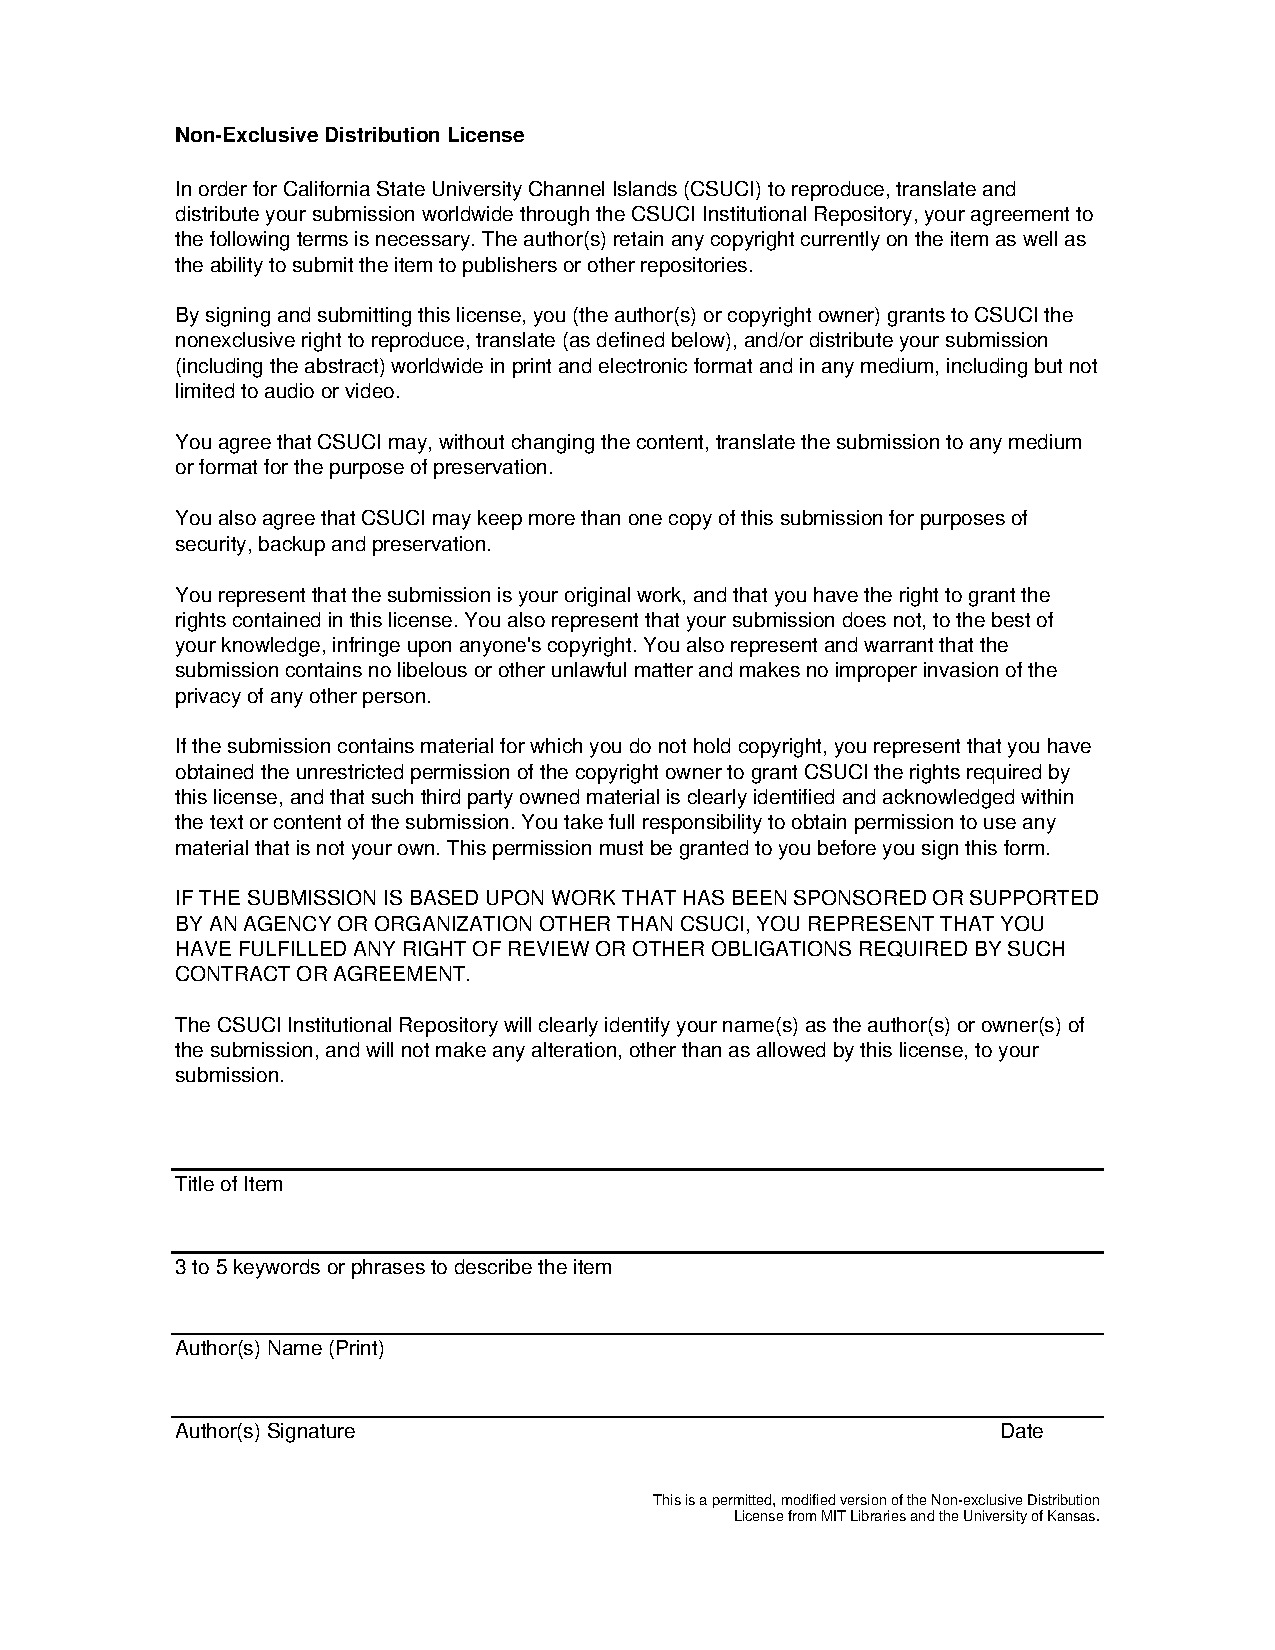
\includepdf{DistributionLicense.pdf}

\newpage

\title{SEAKER:\protect\\A Mobile Digital Forensic Triage Device} 
\author{Eric Elwood Gentry}

\date{\today}
\maketitle

\small{\textbf{Keywords}: Digital Forensics, Digital Forensics Triage, Mobile Digital Forensics,
Digital Evidence, Digital Evidence, Forensic Tools, \gls{rpi}}
\\

\begin{abstract}
As our world of digital devices continues to expand, the potential for digital evidence available to law
enforcement during case investigation is ever increasing.  The growing amount of digital evidence, along with
the deprived pool of Digital Forensic Investigators is causing a backlog to form at many of the digital
forensics labs around the world.  This backlog leads to delays in evidence analysis and reporting, causing
investigators and prosecutors to postpone or even drop on-going cases.\\

The \gls{seaker} device is a digital forensic triage tool that is designed to be simple, portable, inexpensive,
robust, and easy to use.  \gls{seaker} is an acronym for Storage Evaluator And Knowledge Extraction Reader.  
Utilizing a \gls{rpi}, this is a novel approach to helping provide immediate feedback to investigators
along with attempting to stem the backlog problem.  It was originally developed for on-scene investigations
that require immediate feedback, especially in time-sensitive investigations.  It also appears to be an
excellent tool to help reduce the backlog by preventing over-collection of digital evidence.  \gls{seaker} is not
meant to replace a fully-functional digital forensic lab, but instead to augment the initial investigation
and help reduce the backlog.  This research and device overview proposes the mobile, inexpensive, digital
triage device called \gls{seaker}.
\end{abstract}

\newpage
\pagenumbering{roman}

\tableofcontents

\newpage

\printnoidxglossaries

\newpage

\listoffigures

\newpage

\listoftables

\newpage
\pagenumbering{arabic}


\section{Introduction and Literature Review}
\label{sect-IntroAndLitReview}

\subsection{Introduction}
Law enforcement investigations involve many aspects of criminality and need carefully thought-out
procedures and practices.  These procedures and practices are essential to finding the evidentiary
information necessary to determine criminal liability, but are also in place to ensure that the evidence
collected is not tainted and is sound, viable, admissible court evidence.  Establishing and retaining the
forensic integrity of the evidence is a required and crucial part of the investigator's task.\\

Performing investigations is also a noteworthy endeavor.  There are many steps involved that require special
training to be performed properly.  One primary example is the {\em chain of custody}.  This refers to the 
step-by-step documentation record regarding evidence that includes details such as who had custody of
the evidence, when they had custody, who it was transferred to, who analyzed it, etc.
Another is the exacting
science of collecting, labeling, itemizing, and acquiring of evidence.
For instance, collecting physical evidence requires the
use of gloves,
evidence bags, fingerprint-dusting equipment, etc. to prevent cross-contamination, fingerprint smudging,
DNA evidence mishandling, and a multitude of other evidence tainting.  Without the proper adherance to 
guidelines,
even conclusive evidence may not be admissible during a case.\\

Digital evidence is also very essential to many investigations and cases in the modern world.
With each passing year, more and more digital devices are collecting, storing, and uploading data.  As
well, electronic devices for personal use appropriately labelled the Internet of Things (IoT) or
the Internet of Everything (IoE) are becoming more and more
ubiquitous in our everyday lives.  IOT devices are now everyday household items like refrigerators,
thermostats, light bulbs, window coverings, garage door openers, keys, clothes, and much more.
These devices and the massive amount of digital information that
is being generated and collected are often helpful in criminal investigations.  The data can be used to
construct timeframes of activity, locations of individuals, Internet activity, computer users and usages,
and lots other potential digital information.\\

One growing and particularly helpful aspect of an investigation is digital forensics.  This not only 
involves collecting potential digital evidence, but also analyzing, 
and reporting procedures.  This almost always requires a search warrant - a court-ordered search and
seizure of potential evidence of a location where a suspect resides, works, or may be storing it.
The search warrant is executed after it has been obtained from a judge and can involve physical and
digital evidence, as well as other items of consequence.\\

Search warrant investigations are often fraught with danger, intentional obscurity, hidden evidence, and
potential mishandling of evidence.  Before anything else can be done, the location must be considered
secure - considered safe from harming investigators and free of potential threats.  Once a scene is
secured at a search warrant service involving electronic evidence, three activities
take place simultaneously: the search for physical evidence, the search of the physical evidence
itself for electronic evidence, and the interviewing of involved parties.\\

The physical and digital evidence can guide the interviewing of the suspect(s), but also
has the potential to have both positive and negative effects on the
outcome of the investigation. If investigators do not locate any physical evidence for an examiner
to evaluate, then intelligence is not gathered and the interviewer has less information with which
to confront the suspect(s). If investigators present physical evidence to an examiner who is able to
evaluate it quickly in the field, then the interviewer (who is oftentimes also the lead investigator
on the case) can confront the suspects and potentially secure statements that lead to prosecution.\\

This leads to the need for digitial forensics specialists to bring their lab equipment into the field,
especially when serving a search warrant.  The lab equipment is specialized software and hardware
designed to analyze, report, and maintain forensic integrity on potential digital evidence.  This
equipment often involved a laptop, a write-blocking device, media imaging storage devices, expensive
software, and associated cabling for connection and power.  As well, this software is designed for
extensive and in-depth searching and often takes hours or days to analyze the evidence.  Many of the
reports from these systems are designed to be thorough and may take a skilled digital forensic
examiner days to pour over the material produced.  Oftentimes, this equipment is not brought
into the field and all digital evidence is simply collected for later analysis at the law
enforcement facilities.\\

The need for a more field-friendly digital forensic {\em triage} solution will assist in the initial
investigation tasks in multiple ways:
\begin{enumerate}
  \item It enforces a structured procedure and approach that is user-friendly to {\em non-digital
  forensic aware investigators} with the goal of simple instructions for use and very simple 
  evidence location.
  \item It enables investigators, especially interrogators, a very fast digital-evidence overview
  into the types of files
  and information being accessed and stored on the computer equipment at the site of the search
  warrant.
  \item It limits the number of devices and therefore the amount of data required in the in-depth
  analysis phase at the lab.
  \item It minimizes the impact and inconvenience to innocent parties at the site of the 
  search warrant.  The devices that are searched and found to have no evidenciary value can be
  deemed inconsequencial to the case and not be taken into custody.
  \item It may be used to provide initial, albeit simplified, analysis results on potential
  digital evidence ingested into the digital forensic lab.
\end{enumerate}

The topic explored in this paper is a portable, inexpensive, efficient device, named \gls{seaker},
that is intended to overcome the need for a full digital
forensic lab equipment suite to be brought into the field.  The \gls{seaker} device was conceived and 
an initial prototype was produced at the California State University Channel Islands (CSUCI)
campus in a 
Masters level Cyber Security class (COMP 524, Summer 2017) in direct collaboration with the
Southern California High Tech Task Force (SCHTTF) division of the Ventura Country
District Attorney's (VCDA) office.\\


\subsubsection{Author's Contributions}
Author's direct contributions to the \gls{seaker} device project:
\begin{enumerate}
  \item Developed the bash script to turn a standard \gls{rpi} into a
  \gls{seaker} device by programmatically
  installing raspbian software packages, setting up WIFI as a wireless access point, adding a web server,
  and preparing the running environment with the proper fileset
  \item Wrote a custom executable using the C programming language to increase the \gls{seaker} device's 
  searching efficiency in lieu of slower, native operating
  system solutions for finding content on digital media
  \item Co-presented and demonstrated the initial \gls{seaker} prototype for the Summer 2017 Masters level CSUCI
  Security class project to SCHTTF, CSUCI department heads, and local community leaders
  \item Presented the \gls{seaker} device as a thesis project at the April 2018 CSUCI Cyber Security Event
  to CSUCI President
  Erika Beck, California State Assembly Member Jacqui Irwin, Ventura County Sherriff's Department,
  and other local community leaders
  \item Co-authored a conference paper on the \gls{seaker} project and the technology behind it
  \item Updated and enhanced the \gls{seaker} device functionality to support the latest raspbian operating system (Stretch
  Lite, April 2018 release), including enabling ethernet passthrough to the wireless access point
  \item Co-authored by creating Logic Models and assisting with read-throughs for a United States
  Department of Justice (DOJ)
  grant proposal for future work on this project (\gls{seaker}) and
  a second, related security project (Voyager)
\end{enumerate}

\subsection{Literature Review}
\subsubsection{History of Digital Evidence}

The digital forensics field began in the mid 1980s with an understanding from several law enforcement
agencies that computers would play a critical role in future criminal investigations of the future.
In 1993, the FBI hosted an international conference on computer evidence in Virginia.  This was
the first major conference on the subject and had attendees from 26 different countries.  Much
of the original computer
forensics at that time related to recovering information from local computers.\\

Among the early pioneers in the digital forensics field, there was a common understanding that a
system of processes and procedures were needed to locate, record, analyze and report information.
This process would have to be similar to how non-digital physical evidence was handled, but also
include other computer specific preservation methods to ensure the integrity of evidence found.
Those processes and procedures have increased in complexity over time and have suffered from the
lack of unanimous adoption to a single standard.\\

In 2006, Rogers et al\cite{rogers2006computer} proposed a standardization model for a portion
of the entire process called {\em triage} for digital
forensic examiners to follow: Computer Forensics Field Triage Process Model.
The authors of the CFFTPM note the important legal and technical
considerations prior to implementing CFFTPM on a particular investigation.  The legal
considerations include issues
related to search warrant scope and its limitations, U.S. Constitutional 4th Amendment rights, etc.
The technical 
considerations include type of case, criticality of timeliness, skillset of the on-site
digital forensic examiner, 
skillset of the suspect, having proper lab equipment on-site, scene control, etc.\\

Even as late as 2013, Shaw et al\cite{shaw2013practical} points out that neither digital forensic
triage examination nor digital forensic full examination are well defined.
Digital forensic triage may mean something completely different to two digital forensic
examiners.  As well, full digital forensic examination has no robust standard to follow, Although
there has been no shortage of attempts.\\

The National Institute of Standards and Technologies (NIST) published guidelines for several
different types of digital evidence, for instance mobile phones, and computers.
However, NIST focuses on the analysis portion of the science, but leaves the collection,
and reporting aspects unexplored.  The International Standards Organization also published
a set of guidelines, but primarily focused on collection and handling aspects of digital
evidence.  
Ajijola et al\cite{ajijola2014review} provided a thorough review in 2014 of the NIST SP
800-101 Rev. 1:2014 guidelines
titled Guidelines on Mobile Devices Forensics and ISO/IEC 27037 titled
Guidelines for
Identification, Collection, Acquisition, and Preservation of Digital Evidence.
Their recommendation was a combined approach, though still not a fully formed solution.\\

\subsubsection{Process and Procedure Standardization}

Several approaches over the years have been proposed as universal processes and procedures to
gathering, reviewing, and presenting digital evidence.  These approaches range in number of
steps, process coverage, and overall methodology, 
but all have the common goal of finding usable digital evidence for preventing future
harm to society and preserving the potential digital evidence's 
integrity for means of presentation in court cases.\\

In the early years, some research facilities arose to help create and define the processes
and procedures necessary.  Among these were the Computer Analysis and
Response Team (CART), the Scientific Working Group on Digital Evidence (SWGDE), the
Technical Working Group on Digital Evidence (TWGDE), and the National Institute of
Justice (NIJ).  Since their respective inceptions, they have all strived and 
contributed to standardization on approaches and methods for 
the handling and processing of all digital evidence.\cite{noblett2000recovering}.\\

In addition, the United States Department of Justice (DOJ) published 
{\em Electronic Crime Scene Investigation: A Guide to First Responders}
\cite{ballou2010electronic} in the early 2000s that outlines
the necessary four steps for properly investigating digital Evidence:

\begin{enumerate}
  \item {\em Collection}, which involves searching for digital evidence,
  deciphering what should be collected, acquiring the media,
  and chain of custody documentation.
  \item {\em Examination}, which includes searching the digital media
  and attempting to reveal the evidence, especially when it is
  hidden or obscured.
  \item {\em Analysis}, intending to review the evidence for important
  legal infringements. 
  \item {\em Reporting}, for documenting the process used and evidence
  uncovered in the investigation.
\end{enumerate}

The 2003 {\em Integrated Digital Investigation Process} (IDIP)\cite{carrier2003getting},
proposed by Carrier, et al is a model that in their own words:
\begin{quote}
``uses the theory
that a computer is itself a crime scene, called the digital crime scene, and applies crime scene
investigation techniques.''
\end{quote}
It consists of five main phases (in addition, see Figure~\ref{fig:IDIP}):

\begin{enumerate}
  \item {\em Readiness}, for training, preparedness, infrastructure and resources
  preparation before any investigation even begins.
  \item {\em Deployment}, which is intended to capture the process for when an 
  incident requires digital evidence procedures and assignment of resources.
  \item {\em Physical Crime Scene Investigation}, for processing the physical
  evidence from the environment.
  \item {\em Digital Crime Scene Investigation}, for collecting and
  analyzing the digital evidence that exists in the virtual environment.
  \item {\em Review}, for examining the process used in the investigation and
  potential areas for improvements. 
\end{enumerate}

\begin{figure}[ht]
  \centering
    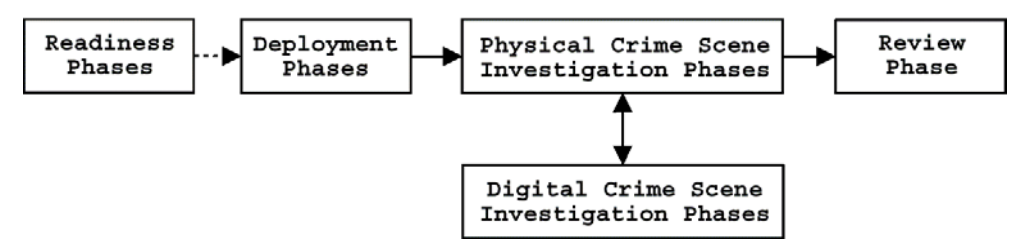
\includegraphics[width=0.8\textwidth]{images/IDIP.png}
  \caption{Integrated Digital Investigation Process Model (IDIP)}
  \label{fig:IDIP}
\end{figure}

Baryamureeba and Tushabe\cite{baryamureeba2004enhanced} proposed a model based
on the best parts of the US DOJ's {\em Electronic Crime
Scene Investigation}, the {\em Abstract Digital Forensics Model}, and 
the IDIP model.  Their proposal was called the
Enhanced Integrated Digitial Investigation Process (EIDIP).
Their model was proposed in 2004 at the annual Digital Forensic Research conference
(DFRWS)\cite{baryamureeba2004enhanced} and included the following phases:

\begin{enumerate}
  \item {\em Readiness}, same as IDIP.
  \item {\em Deployment}, which encompasses the Deployment,
  Physical Crime Scene Investigation, and Digital Crime Scene
  Investigation phases from IDIP.
  \item {\em Traceback}, that includes connecting the evidence collected
  in the previous phase to the suspect(s).  Typically this is done with IP
  addresses and requires the authority to gather this information.
  \item {\em Dynamite}, which includes the reconstruction of the events
  suggested by the evidence and  the documentation and submission to the
  appropriate legal authories.
  \item {\em Review}, same as IDIP.
\end{enumerate}

In 2006, Rogers et al\cite{rogers2006computer} proposed a reliable, repeatable process 
model designed specifically for digital evidence triage called
Computer Forensics Field Triage Process Model (CFFTPM). It was created in partnership
with Purdue University's Cyber Forensics and Computer and Information
Technology Departments, along with the National White Collar Crime
Center\cite{rogers2006computer}.
The process was derived from several other military and law enforcement models
including IDIP, 
Digital Crime Scene Analysis (DCSA),
and a military Operations Order (OpOrd).  In coordination with the Southern Indiana 
Assistant U.S. Attorney's office,
USADA Steve Debrota, Rogers et al\cite{rogers2006computer} implemented and reported
on the success of their proposal.  This amalgamation of approaches is still inspiring 
the latest trends in Digital Forensic approaches.\\

Shaw et al\cite{shaw2013practical} analyzed the ACPO and focused on the second step (Capture)
as the primary guideline for evidential integrity.  They strongly suggest compliance with
digital forensics best practices, like the ones provided in the ACPO.  Their final approach
and recommendation was to combine Linux utilities with a simplistic interface to standardize
the output and enable investigators who may not have full digitial forensic backgrounds
to perform triage on potential digital evidence.\\

The Association of Chief Police Officers (ACPO), a private company that helped establish and
develop policing practices in England, Wales, and Northern Ireland for many years,
put together a {\em Good Practice Guide for Digital Evidence}\cite{williams2012acpo} in 2012 that outlines some
recommended procedures for dealing with digital evidence.  As with other methodologies, this guide
explains utilizing a four step approach: Plan, Capture, Analyze, Present.\\

The ISO/IEC 27037 guidelines provide an attempt at an internationally 
recognized approach,
with the goal of making it easier to compare, combine, and contrast
results for out-of-jurisdiction cases and for data scientists' research.  It provides a
common reference line for 
digital forensics\cite{ajijola2014review}.  However, it is not meant to replace laws or regulations.
The main purpose is to provide practical
assistance for investigations involving potential digital evidence, while preventing digital
evidence corruption.  This
process facilitates the usability of evidence by other jurisdictions.  This guideline provided
four steps for handling
potential digital evidence: Identification, Collection, Acquisition, and Preservation.  However,
this is incomplete, as
it only addresses gathering, not actually evaluating or providing results to law enforcement
investigators.\\

All of these approaches are intended to help find and gather digital evidence.  They are also intended
to maintain the forensic integrity.  Some organizations combine these approaches into a system of
processes and procedures intended for use in their own facilities.  Unfortunately, many organizations have
home-grown solutions passed down from senior members of the digital forensics team to the newer
team members.  Not having a universally recognized and accepted standard 
leads to complications and difficulties when digital evidence needs to be shared across other
jurisdictions and boundaries\cite{ajijola2014review}.\\

\subsubsection{Aquisition Methodology}

[MOVE THIS TO THE NEXT CHAPTER!!!!]
The \gls{seaker} tool is designed specifically for the {\em triage} phase of digital forensic
investigations.  As a general approach, this research splits the act of dealing with digital evidence into two
separate methodologies: {\em aquisition} and {\em analysis}.  These are the main foci since \gls{seaker} is 
designed to do both in a very timely fashion and are the main focus of this research.\\

Aquisition has multiple definitions across
the digital forensic universe, but in this case it is meant to imply the entire set of processes and
procedures from training the digital forensic examiners and \gls{seaker} users,
to collecting the media that potential digital evidence may be stored on, 
to the \gls{seaker} usage for gathering the information about each device.\\

The aquisition phase specifically highlighted here is the gathering of physical digital
media and the capturing of potential digital evidence in the triage environment.  The 
setup and training materials for creating and using the \gls{seaker} device are referenced in
the appendix.\\

The analysis step will be discussed in the next section.\\



\subsubsection{Analysis Methodology}

The {\em Analysis} methodology is considered the second phase in the \gls{seaker} approach and 
can consist of both the {\em triage} analysis stage and the {\em full} analysis stage.
Specifically, this paper and the \gls{seaker} device focus on the triage stage of Analysis.  This
stage can be applied in the field or at the digital forensics lab, while the full analysis
is unlikely to be accomplished in the field.  A full analysis could take many hours or days
and is not the first priority when serving a search warrant.\\

However, digital evidence triage is a very useful part of an investigation and can be 
implemented using the \gls{seaker} device.  The triage analysis stage is considered in this research
to consist of an interactive web page that detectives and investigators can use to 
lookup search terms from the digital evidence collected from suspect devices plugged into the
\gls{seaker} device.\\

Rogers et al\cite{rogers2006computer} research in 2006 covered the primary machine type at
the time: the standard Windows machine.  Unfortunately, this leads to an outdated model over
time, since the processes and procedures become obsolete as new technology arises.  Along with
the proliferation of IOT devices, new technologies also have emerged as more mainstream that
need to be incorporated into a more generalized approach.  Some operating systems are being
utilized on a more regular basis, like Linux and Mac.  In fact, even our \gls{seaker} device is
an IOT device based on the unix spin-off of Debian.\\

Ajijola et al\cite{ajijola2014review} - The NIST guidelines provide an in-depth look into mobile
devices, helping to explain the technology involved and its
relationship to the forensic process.  NIST itself is a technological, non-regulatory federal agency under the U.S.
Department of Commerce.  The NIST process model labeled NIST SP 800-101 lays out the digital evidence procedures in
four steps: Preservation, Acquisition, Examination and Analysis, and Reporting.  These four steps provide the
necessary steps for the digital evidence process model as a suggested way to evaluate mobile device information.  This
is useful, but not complete for law enforcement investigators.\\

\subsubsection{Combined Aquisition and Analysis Methodologies}
Hitchcock et al\cite{hitchcock2016tiered} has proposed and evaluated a ``tiered forensic methodology'' model that defines
a process of digital forensic triage utilizing non-digital evidence specialists.  In their research, they identified
a large and growing backlog of digital evidence.  This backlog has led to problems in the law enforcement community
with regards to collecting, analyzing, reporting, and prosecuting.\\

The next tier is when the already-triaged digital evidence is sent for full evaluation.  This is a certified facility
that can perform full digital forensic analysis, called a Technological Crime Unit (TCU).  The TCU is currently
heavily inundated with cases needing analysis and reporting of digital evidence.\\

This tiered approach is based on a Computer Forensic Field Triage Process Model proposed by Rogers et al
\cite{rogers2006computer} and the internation standard ISO 27037 (Information Technology - Security Techniques - 
Guidelines for identification, collection, aquisition, and presentation of digital evidence). The process model 
breaks down the six phases of digital evidence categorization, which Hitchcock et al\cite{hitchcock2016tiered} loosely
based their four phase approach on.  The four phases are: planning, assessment, reporting, and threshold.  The ISO
27037 standard specifically attempts to address the need to minimize the risk of potential digital evidence being
spoiled by mishandling, while also attempting to maximize the evidentiary value of digital evidence collection.\\

This approach is not without risks.  One concern is the accidental exclusion of an item of digital evidence that is
important to the investigation.  Another is the level of computer skills and training of the DTF expert.  The paper ???
does attempt to mitigate the latter with training and management process, while providing evidence that the former
is a common misconception in most cases.\\

Shaw - One example is to note encrypted compressed files for review later.\\

Rogers - This process in no way supersedes the ability or need to perform a full forensic examination at a full-featured
digital forensic lab.\\

Ajijola et al, 2014\cite{ajijola2014review} also proposed a new process
model that is a hybrid of both models with the resulting combination being much more effective than either of its 
individual parts.\\

In the research for combining the NIST and ISO guidelines, Ajijola et al\cite{ajijola2014review} explores the
commonality, differences, and limitations of each model.  Although both models follow the Auditability,
Repeatability, Reproducability, and Justifiability requirements, as well as the Confidentiality, Integrity, and
Availability standards, they individually lack some necessary phases to enable them to be used separately.  The NIST
process model lacks the Identification and Collection phases, while the ISO process model lacks Examination, Analysis,
and Reporting aspects of a full Digital Evidence processing model.\\

The combination of these two approaches, as suggested by Ajijola et al\cite{ajijola2014review}, provides a new five 
step approach: Identification, Collection and Acquisition, Preservation, Examination and Analysis, and Reporting.
These steps provide a more comprehensive approach that law enforcement can use to fulfill its evidenciary duties in
an investigation.  When both process methods are used, the goals approach a full set of tasks from initial on-scene
evalutation to the end of the in-lab digital forensics investigation.\\

\subsubsection{Digital Evidence Backlog}
IDC forecasts that by 2025 the global datasphere will grow to 163ZB (see Figure 1) (that is a trillion gigabytes).
That's ten times the 16.1ZB of data generated in 2016. All this data will unlock unique user experiences and
a new world of business opportunities.\\

\begin{figure}[ht]
  \centering
    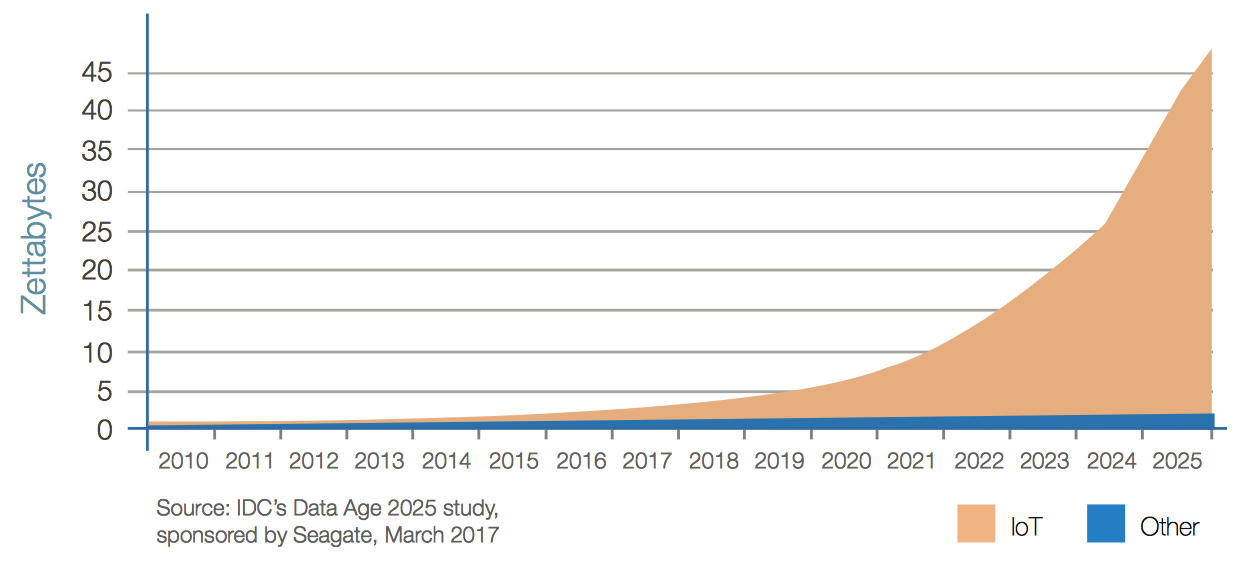
\includegraphics[width=0.8\textwidth]{images/IOT_chart.jpg}
  \caption{IOT Device Data Growth}
\end{figure}

Some of the current challenges in digital forensic investigations are directly related to the amount of data being
created.  As Lillis et al\cite{lillis2016current} explores in their research, there are three main factors
involved in the digital forensic backlog: increasing number of devices seized per case, increased number of cases
involving digitial evidence, and the increasing volume of data per digital media.  This has lead to a growing
and already substantial backlog in digital forensic investigations.\\

One effect of this increased delay and backlog is that cases become inactive, waiting for new leads.  A more
aggressive approach to solving the backlog could help prevent dismissals, cold cases, and potentially more
societal harm from a corrupt investigation suspect.\\

Raghavan\cite{raghavan2013digital} has accumulated a list of 5 major challenges that the digital forensics 
community is facing and continue to add to the backlog problem.\\

The first is the complexity of binary data aquisition, i.e. low level data aquisition through digital media
duplication.  This challenge causes the need for sophisticated data reduction techniques.\\

Another complexity is the diversity of data and lack of standard examination techniques.  The plethora of
operating systems and file formats has been increasing and is posing a more and more significant challenge
over time.\\

The consistency and correlation problem is yet another challenge.  This is a problem resulting from the current
digital media investigation tools not providing the entire picture to investigators.  Only part of the whole
picture is provided when these tools find digital evidence.\\

Another issue that Raghavan\cite{raghavan2013digital} proposed is the volume of data to sort through.  The sheer
amount of data that exists per user is increasing at an alarming rate [cite?], and has lead to a very large
backlog of digital evidence to investigate.  These delays have even caused some cases to be dismissed.  This
challenge is exacerbated by the lack of adequate automation for digesting the data.\\

The fifth, but certainly not the last, challenge proposed by Raghavan\cite{raghavan2013digital} is the timeline
synchronization issue with digital evidence.  Since the evidence could be collected in different time zones, 
with different timestamp formats, clock skew, etc, lining up the events in order can be challenging or
infeasible.\\

With the proliferation of Internet Of Things (IOT) devices and cloud storage, the field of digital forensics
continues to expand.  These areas pose a great challenge, but also new opportunities.  Lillis et
al\cite{lillis2016current} researched cloud storage and found some areas of opportunity, for instance parallel
processing, distibuted computing, GPU/FPGA utilization, and others.  These areas for increasing the efficiency
of ditigal forensics can be explored further due to the substantially reduced I/O limitations in cloud storage.\\

The Internet of Things (IOT) also poses new challenges.  IOT devices are estimated to number near 40 billion by
2020, contributing to the overwhelming amount of digital data.  Since these devices tend to have more 
non-persistent memory and less storage, this causes added complexity for gathering and analysis.  In addition,
a portion of IOT devices are battery operated and computationally challenged, leading to loss of data over
time.\\

Hitchcock et al\cite{hitchcock2016tiered} - The backlog and delays in case reporting are contributors to a common problem of time sensitivity.  Some countries 
have given their citizens a right to a ``speedy'' trial.  As well, some countries have statutes of limitation (limits
on how long after the crime was committed to resolve the case) for most crimes.  Some administrative situations are
also contributors, for instance case prioritization based on chronological filing, crime severity, or victim needs.\\

\subsubsection{Digital Evidence Triage}
The summary of the research done by Hitchcock et al\cite{hitchcock2016tiered} are as follows.  They sought to expedite
the process of sending digital evidence for analysis and results.  One of their goals is to enable more field triage
of digital evidence to reduce the amount collected, and act specifically on pertinent information only.  They 
recommended that some front-line crime scene investigators (non-forensic analysts) be trained in the implementation
of digital evidence triage and evaluation.  These trained individuals would be Digital Field Triage (DTF) experts and
have the ability perform field-level digital evidence triage.  This triage would specifically weed out the benign
from the consequential digital evidence with high certainty, while also protecting the digital evidence from spoilage
and preserving evidentiary integrity.\\

One digital evidence triage method proposed by Shaw et al\cite{shaw2013practical} seeks to standardize on an 
approach they call ``enhanced previewing''.  Enhanced previewing seeks to solve some of the problems associated with
typical triage approaches.  As is the case in other research, Shaw et al\cite{shaw2013practical} extolls the 
need to reduce digital forensic evidence analysis backlogs, especially with the evolution of big data and the
proliferation of digital devices.\\

The proposal for a practical and robust methodology by Shaw et al\cite{shaw2013practical} aims to stem the concerns
of a typical triage process.  Risks still exist, for instance overlooking digital evidence, but it is argued that
those risks are outweighed by the risks of a lengthy process due to large backlogs and the associated delays in
evaluating that evidence.  Another concern exists that inadequately trained people will be charged with performing
on-site digital evidence triage and mishandling or incorrectly evaluating results will cause evidence spoilage.
Other concerns are the potential high cost of software and training.\\

In order to provide a simple, yet robust mechanism, Shaw et al\cite{shaw2013practical} starts with an open source,
CD-bootable image of GNU/Linux and enhances its features to include boot-time application launching, and a simple
to use interface with minimal ability to deviate from task.  This bootable CD is intended to be placed into 
evidenciary computer systems and booted using a series of BIOS modifications or boot-time interruptions.  This 
mechanism to boot the system off of a bootable CD is difficult, and where the most problems with untrained users
of the enhanced previewing will happen.\\

The enhanced previewing concept has valuable merit, in that the collection mechanisms are thorough.  Using the
GNU/Linux based system and having written code for it, Shaw et al\cite{shaw2013practical} utilized some well
thought-out approaches.  First, all hard drives from the evidentiary system are mounted into the GNU/Linux
filesystem as read-only, thereby eliminating the need for write-blockers.  As well, the entire hard drive is
evaluated, including the file system, all partitions, unallocated space, deleted files, and compressed files.  In
addition, other mechanisms are employed that continue to enhance the previewing are employed.\\

Rogers - The CFFTPM was created to enhance the investigators ability to obtain useful information at execution time of a 
warrant at the suspect's dwelling or work.  The process is designed to be used in the first few hours of the 
investigation, especially during the first suspect interview and search execution phase of the investigation.  It is
known that suspects are more likely to divulge more information and be more cooperative in that environment (Yeschke
2003\cite{yeschke2003art}).  As well, location of and presentation with suspect ``triggers'' from the potential evidence
increase the suspect's willingness to talk and cooperate while on site.\cite{rogers2006computer}\\

The foci of the CFFTPM are immediately finding usable evidence, identifying victims at acute risk, guiding the
on-going investigation, identify potential charges, and accurately assess the offender's danger to society.\\

Rogers - The CFFTPM is broken up into phases, two of which have sub-phases (see Figure 2).  The main phases consist of Planning, Triage,
Usage/User Profiles, Chronology/Timeline, Internet Activity, and Case-Specific Evidence.   Usage/User Profiles are broken down into three sub-phases:
Home Directory, File Properties, and Registry.  These are important and help distinguish user specific activity and
permissions.  The Internet Activity phase is also broken down into three sub-phases: Browser Artifacts, Email
Artifacts, and Instant Messenger Artifacts.  These also help establish user activity.  Some importance is explicitly
stated to skip based on type of investigation and prioritizing the investigation.\\ 

\begin{figure}[ht]
  \centering
    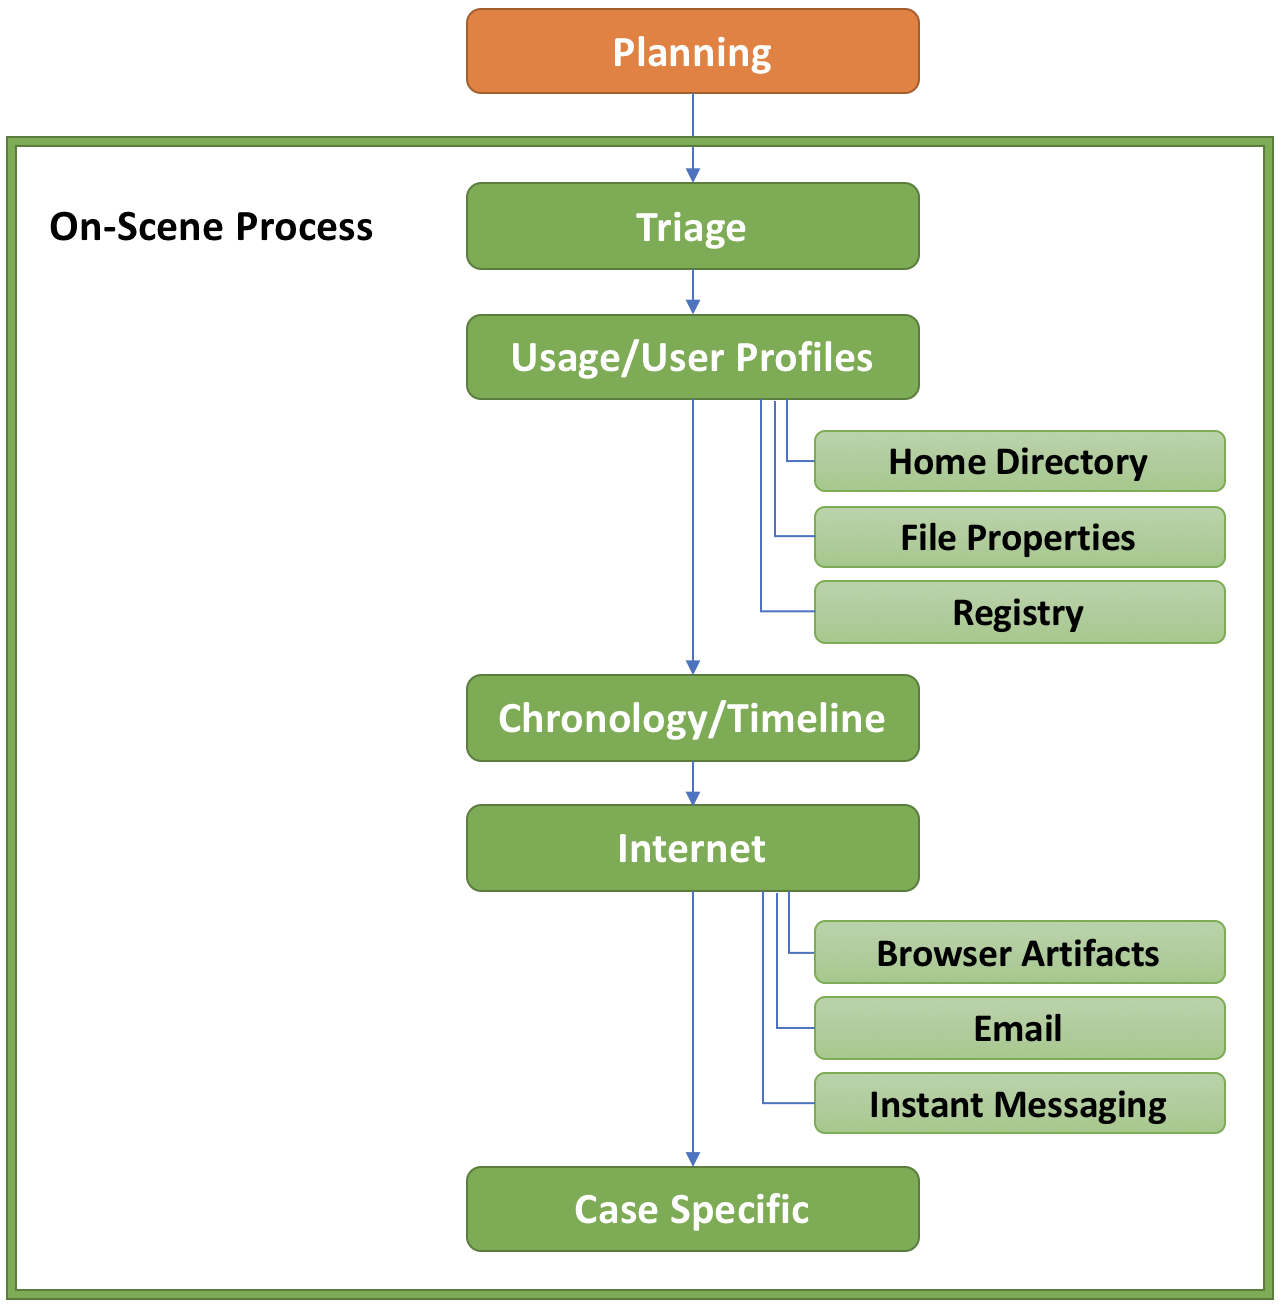
\includegraphics[width=0.8\textwidth]{images/CFFTPM.png}
  \caption{Computer Forensic Field Triage Process Model (CFFTPM)}
\end{figure}

\subsubsection{How \gls{seaker} Can Help}
The research of Hitchcock et al\cite{hitchcock2016tiered} should be referenced for a good process starting point for
digital forensic labs.\\

Rogers -  This is where the \gls{seaker} portable
triage device can help by evaluating every aspect and prevent the on-site investigators from skipping or
de-prioritizing critical potential evidence.\\

Rogers - This is also an area where the
\gls{seaker} portable triage device can help eliminate some of the potential problems, for instance technical prowess of the
on-site investigators and proper lab equipment on-site.\\

Rogers (CFFTPM) - Some particular aspects of the phases are critical to investigators in revealing evidence or potential evidence for
the \gls{seaker} portable traige device.  Usage/User Profile information is extremely important.  This includes the need to
be able to view and search files, folders, registry keys, and file properties associated with a particular user.  The
Internet Activity artifacts also become very useful, especially in the case of child pornography.  The browser, email,
and Instant Messaging artifacts can lead directly to potential charges.  Finally, a Chronology/Timeline understanding
and ability to sort based on it can significantly narrow down the possibilities of which user information and which
Internet Activity is the most important and critical to the investigation.\\

Rogers (CFFTPM) -Implementing this in the \gls{seaker} portable triage device is crucial for simplicity and ease of use.  As well, it goes a
long way towards having an implementation of \gls{seaker} being understood and adopted.  Reporting is also a critical need
and is implemented in a way that will enable digital forensic investigators to provide early information to
investigators and prosecutors.  This helps alleviate the need to wait until the backlog of digital evidence is cleared
to get any information from case-specific digital evidence.\\


\section{Background}
\label{sect-background}

In a labratory environment, digital forensics investigators have the ability to discover
a tremendous amount of material that is potential evidence.  This includes anything 
digitally stored on the evidentiary media from
explicity illegal files to IP address connections to a digital chronology of
events.\cite{raghavan2013digital}\cite{rogers2006computer}
The software and hardware necessary to perform the
in-depth, full evaluation of the media are specialized for digital forensics 
work, but typically are costly, don't travel well, and can take many hours for
results from a single digital media device.\\

In the field environment, digital forensics
investigators are likely to not have the time, equipment, or proper environment to
obtain evidence from the digital devices found during the execution of a search
warrant.  In some cases, due to various reasons, digital forensics investigators
are not able to attend and therefore all of the digital media is taken into
custody for analysis at the digital forensics lab.  When they are able to attend,
they typically
bring a subset of their lab environment with them to start deciphering
the digital information and attempt to perform a traige analysis.\\

In a coordinated effort with SCHTTF, this research is an attempt to help
solve some of the field environment limitations of digital forensics investigators.


\subsection{Legal Details}
In order for digital forensic investigators to obtain the data from a digital device,
a search warrant for that device must be obtained.  As well, law enforcement must
obtain a search warrant to acquire the device for searching in the first place.\\

Search warrants are necessary for law enforcement to obtain crucial evidence in many
cases.  A search warrant is obtained by a judge's order.  Law enforcement must 
provide probable cause that a crime 
was committed and that items connected to that crime are likely to be found 
in the place specified by the warrant.  The judge will review the matter and if
they are in agreement, will authorize law enforcement to search a particular location
for specific items which are declared in the search warrant.\\

When law enforcement aquires the digital devices for an investigation, there is
an important document that must also accompany them.  This is called the chain of
evidence or chain of custody, which is used to track who currently has control
of the evidence and
who has had control chronologically since it was originally seized.
The information in the chain
of evidence is date, time, and location of acquiring, securing authority, and who is
gaining posession of the device(s).\\

After a digital device has been acquired by digital forensic investigators, they
must take special care not to alter the device's information in any way.  This 
requirement figuratively mimics the care a physical forensic investigator must
take to preserve physical evidence.  Special processes must be followed to ensure
that the potential digital evidence is not altered and, in fact, must be able to 
be proven if the matter ends up in a trial.  This is critical to ensure that the
evidence obtained from the device is admissible in court.\\

One device to aid in the proper handling of digital evidence is called a
write-blocker.  Digital forensic investigators use this device as an intermediary
between the devices and the computer systems they plug the devices into for
investigation.  The typical first step when a device is acquired by a digital
forensic lab is for the device to imaged (or copied bit by bit) so that the
image can be used for further evidence searching.  This provides an extra level of
abstraction, so that the actual device is kept in pristine digital condition.\\

Write-blocking has been implemented in digital forensics labs with an in-line 
piece of hardware.  Companies like Guidance Software and others have created
write-blocking devices that are added to the list of hardware necessary to 
prevent modification of any kind to the potential digital evidence.  The Tableau
product line is a great set of these types of devices.  Although they are made
to be simple and easy to use, they create yet another piece of the lab that must
be carried into the field and required to be plugged in and used.\\

For this research, the SEAKER device is intended to be used for triage investigation
on digital devices to perfom an initial search for potential digital evidence.
Instead of having a separate write-blocking device, the \gls{rpi} is setup with
write-blocking capabilities when digital devices are connected to it.  This
configuration enables the SEAKER's own system to act as a software-write-blocker
to prevent any digital alteration to the device.\\

\subsection{Technical Details}

Choosing the \gls{rpi} as the base platform for the SEAKER device was intentional
and guided by some of the principals of the originating company.\\

\gls{rpi} is manufactured by the Raspberry Pi Foundation in the United Kingdom
for the purpose of teaching Computer Science in schools and around the world.  It
is a fully functional CPU with RAM, input and output connections, status lights
and the ability
to be powered by batteries, USB, or an electrical wall socket connection.
The form factor is small and the cost is kept to a minimum for ease of
aquisition, use, and adaptability.  As of this writing,
the most powerful version of the \gls{rpi} is \$35.  Uses for the \gls{rpi}
device are numerous and growing.\\

The SEAKER device project is yet another adaptation of how the \gls{rpi} device
can be utilized from concept to fully featured digital evidence triage device.\\

Another goal of the SEAKER project is to enable investigators without 
digitial evidence training or with limited computer training to utilize it
on-site at the execution of a search warrant.  The SEAKER device is designed to
be self-sufficient and automatically self-preparing when it is plugged into a 
power source.  The device will boot, prepare the web server, the wifi hotspot
and be enabled to handle digital devices that are attached to its USB port.
Once a digital device is plugged in, it is automatically mounted and scanned.
A web-page interface was created for accessing the scanned devices when a portable
wifi-enabled phone or tablet are connected to SEAKER.\\

These attempts to make the process as simple as possible are intentional and 
make the process of digital evidence triage collection and searching accessible
to investigators with or without specialized computer knowledge or training.\\

Some specialized training is available to those investigators who want to 
become digital forensic investigators.  The typical learning takes place over
a full year of classes and hands-on work through one of several federal or 
law enforcement agencies.  These lead to certifications like Digital Evidence
First Responder (DEFR), Digital Evidence Specialist (DES), or Digital Forensic
Investigator (DFI).\\

\section{Development of \gls{seaker} Device}
\label{sect-developmentSeakerDevice}

The SEAKER device concept is very novel, not only in its capacity as a digital 
forensics evidence triage device, but also in the fact that it is low cost, highly
available, simple to setup and use, and provides very fast results.\\

There are other digital triage tools on the market, but almost every one is a
software solution that involves either a separate laptop or a bootable
CD, DVD or USB drive to enable the interaction.  These types of software tools
typically require advanced computer knowledge and a digital forensics specialists
to be involved.\\

Since the SEAKER device project was a collaboration with SCHTTF, it already has
built-in law enforcement acumen related to digital forensics.  As a digital
forensics evidence traige device, it could be shaping the way investigators
handle computers and other digital equipment during execution of a search warrant.\\

\subsection{Conception}

The SEAKER device project came to be in the Masters level Cyber Security class (COMP 524)
at CSUCI in the Summer semester of 2017.  It was proposed to the class by professor 
Dr. Michael Soltys during one of the initial lectures as the final project for the
course.  The attending students agreed and work began on it, in addition to the other
assignments due in the course.  Dr. Soltys broke down the problem into categories so
that teams could form and work on each piece individually.  The categories were:

\begin{itemize}
  \item Connecting hd to a RP/NUC, sensing OS and mounting (2 teams together)
  \item Searching in the mounted file system (2 teams together)
  \item Sending report to an iPad/laptop/handheld
  \item Documentation and troubleshooting
  \item Testing
\end{itemize}

This breakdown helped guide each team to get started on their contribution to the
final project.  However, before the students could begin, the device platform to use,
the technological method for input and output, and the feature set had to be agreed on.\\

The device platform chosen was the \gls{rpi}.  This enabled the students to work on the platform
independently, due to the inexpensive nature of it.  As well, two \glspl{rpi} were provided
for the classroom by SCHTTF and Dr. Soltys, respectively.\\

The input method chosen was setup for two types of input.  The first type was connecting
the digital devices to the SEAKER device.  This was agreed upon to be either with the USB
port that was built into the \gls{rpi} or via a USB to SATA converter cable.  This enabled
the digital device to be mounted by the Raspbian Operating System and automatically 
searched for content via the mounting rules.  The second type of input was human input
for a set of terms to search.  The search terms were agreed to be put into a web form that
would be submitted to the on-board web-server.\\

The output method clearly needed to match the input method in terms of technology, so the
use of the on-board web-server was chosen to be the output method.  When investigators are
using the SEAKER device, they would be shown a webpage asking them to submit a 
set of search criteria.  The results would be given back to the phone or tablet in HTML.
This also enabled quick building of the HTML framework and response mechanisms.\\

Finally, the feature set needed to be agreed to.  With direct guidance from the SCHTTF,
specifically Frank Lyu, the class agreed to the following:

\begin{itemize}
  \item Write-blocking of attached digital evidence devices
  \item SATA and USB storage devices
  \item FAT, NTFS and EXT* file systems to be read from storage devices
  \item Filename-keyword filter
  \begin{itemize}
    \item Prepopulated keyword list
    \item Customization of keyword list
  \end{itemize}
  \item Status lights for power, and device status
  \item Wireless connection to a phone or tablet for keyword input and results
  \item Ability to find and display search results and digital device hardware information
\end{itemize}

The proposal for the SEAKER device project initially came from the SCHTTF.  They wanted
a device that could quickly ascertain potential evidence and enable on-scene investigators
to search devices while questioning suspects.  This process of searching the digital devices
immediately is called triage.  With it, investigators are able to provide actionable
intelligence quickly, prioritize devices to be previewed, reduce preview setup time, and
triage larger amounts of devices.\\

\subsection{Setup Script For \gls{rpi}}

The idea of a setup script for the \gls{rpi} was conceived early by the author, since
each team was assigned to work independently and the deadline of implementation was
extremely short.  This was, after all, a summer class.  In order to get everyone in
the class up and running and able to do work on their individual pieces, there
needed to be a baseline for everyone to start working with.  Starting with the 
base operating system image, called Raspbian, the setup script was meant to modify
it to handle the scenarios we were attempting to create.\\

First, there needed to be some initial setup for keyboard, timezone, SSH, hostname,
and installing some additional packages.  To prevent unnecessary 
software from occupying the local Micro SD card, the ``lite'' version of Raspbian
was chosen as the base operating system.  However, that meant that additional
Raspbian packages needed to be added; for instance, the Apache web server, a DHCP
server, PHP, the software to convert the wireless NIC card to an access point, and
the device drivers for FAT32, NTFS, HFS, EXT*, etc.\\

Next, the setup script needed to customize the SEAKER device based on user
parameters.  These include hostname, IP address, DHCP supported range, Raspbian
user {\em pi}'s password, and the wireless access point password.\\

The setup script then prepares the \gls{rpi} access point configuration, web server
configuration, mounting rules, default web-pages, and compiles the custom C code
for searching (listed in appendix).\\

Finally, in order to avoid simple hacking and password locations, the setup
script clears the history, sets itself up to be deleted at boot time, and removes
any other reminants from the original setup.\\

Most of this was done by the author and published to the class so that they could
begin using the \gls{rpi} as a SEAKER device and begin their work to implement the
rest of the functionality.

\subsubsection{Web Server}

The Apache web server was chosen, since it is a standard Unix-based operating system
choice for serving web pages.  It also supports backend coding opportunities when 
coupled with a server-side code execution program like PHP.  Setting this up was
included as a part of the setup script.\\

A couple of steps were needed to implement the web server.  The first was to
load the Apache and PHP packages coinciding with the Raspbian operating system.  
Since it is a branch off of Debian operating system, these were easily found and
worked well.  The next step was to load all of the files that were needed for
the HTML and PHP to display and operate properly.  The final step was to modify
the access to each of the files to be specifically accessible by the web
server daemon account.  This was necessary to ensure the files could be read and
served up by the web server when requested.\\

In addition, the {\em collection} code for searching the drive needed to have 
access to a shared location for the filename and folder searching algorithm.
The {\em \textbackslash{}tmp} folder was chosen as a suitable location, since
both the collection program and the web server have access to it.  An extra
feature of using {\em \textbackslash{}tmp} is that the operating systesm clears
out the entire folder everytime it boots up, causing the previous data to no
longer show up.\\

\subsubsection{WIFI Setup}

The wireless NIC also needed to be setup to be a wireless access point so that
investigators could connect with a phone or tablet and use the web page access
to perform searches on the digital devices.  The main idea here was to have a 
password-protected closed network where the potential evidence could be searched.
This was included as a part of the setup script.\\

The steps involved here were complicated and difficult to setup properly.  As
with the web server, the proper Raspbian operating system packages needed to be
acquired and installed.  In addition, the setup of those packages required 
setting up DHCP, WPA, the wireless NIC, and the access point daemon.  Setting
these up mainly required adding and altering text configuration files.  
Unfortunately, the Internet was not much help, leading to a lot of trial and 
error testing to make sure it all worked.\\

Finally, this process required a reboot, which was able to be postponed until
the end of the setup script.\\

\subsection{Rules For Mounting}

During the setup script for the SEAKER device, auto-mounting is setup to
automatically mount new digital media devices that are plugged into the USB
port.  Another script was written to handle the post-mounting {\em collection}
of the applicable drive contents.  The post-mounting script is also
configured to run once any new digital media devices are plugged in.\\

In order to accommodate the request to ensure the forensic integrity of the
suspected digital evidence, special mounting options were required.  There
are two different aspects for how a drive can be written to.  The first is
the standard {\em writable} option, which allows the content of files and
folders to be created and modified.  The second is called {\em journaling},
which is an operating system concept for logging when and what the OS 
did to the drive.  Both options, {\em ro} and {\em noload}, are applied to
the mounting options.  This makes the SEAKER device functionally consistent
with a write-blocking device, as mentioned earlier in Chapter 2.\\

\subsection{Code for Searching Device}

The code for searching the digital devices was specifically aimed at gathering
every filename and location into a searchable file and storing it so that
those drive contents could be searched, even after the digital device had been
disconnected from the SEAKER device.\\

There were several options for searching for files.  The simplest way is to use
the built-in operating system mechanisms, for instance {\em ls} or {\em find}.
Another way is to code a simple C program that does the same thing.  There is
another built-in operating system mechanism that is much faster when used on
standard unix-based environments called {\em locate}, however, that utilizes
an index that is built up over time and does not work well with newly
attached devices.\\

Since one of the goals of the SEAKER project was speed of collection, a test
was performed that
measured the built-in mechanisms vs the simple C program.  The simple C program
was by far the fastest, beating the other two methods by an average of 26\%
(see Table~\ref{tab:CollectionAlgorithmData} for data).
My theory on why is that the other programs have many
built-in options and functionalities that are not utilized.  However,
those extra functionalities have unnecessary code switches and therefore extra
execution paths that are not necessary for this file and directory collection
application.\\

\subsection{Web Code}

HTML and PHP were chosen as a simple interface for quick development.  It also
allows for easy access via many different devices through a standard web 
browser.\\

The main page (Figure~\ref{fig:MainPage}) was designed to be very easy to use
and as automatic as possible.
The list of searchable devices is populated at the load-time of the page.  As
well, the page refreshes itself until searchable media is found.  The 
default keyword search list is also shown on the page.  Each keyword is
searched independently and are entered one per line on the input keyword
text form.  The keyword search list is read in using
PHP from a pre-determined file that resides on the Micro SD card.\\

\begin{figure}[H]
  \begin{center}
  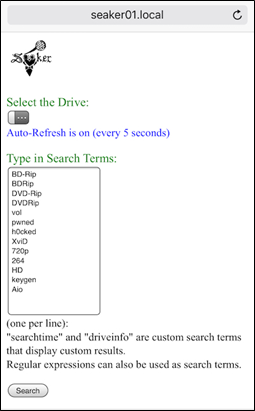
\includegraphics[width=6cm]{images/seaker-hh-screen-2.png}
  \caption{Main Page}
  \label{fig:MainPage}
  \end{center}
\end{figure}

When triggered using a {\em Search} button, the media list and the
keyword list to search are passed to the web server via a webpage POST.  The
results page is then dynamically created using PHP to read each media's file
and directory list and write the matching results to the returned webpage.
The Raspbian operating system built-in command {\em grep} is utilized to
find the results on the server side.\\

The resulting page (Figure~\ref{fig:ResultsPage}) is then displayed to the user 
using a simple HTML expand/collapse tool.  Each media searched and each search
criteria are accessible via this tree-like tool.\\

\begin{figure}[H]
  \begin{center}
  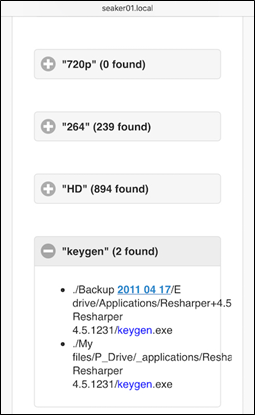
\includegraphics[width=6cm]{images/seaker-hh-screen-3.png}
  \caption{Results Page}
  \label{fig:ResultsPage}
  \end{center}
\end{figure}

In addition, some special keywords can also be used to obtain information
about the media.  The search term {\em driveinfo} can be used to list the exact details of
the media, including serial number, size, and other information.
The search term {\em searchtime} can also be used to show the time needed to find the
full drive information as well as the time for the particular search.\\

An administration page was also created for editing the default search keywords.
This page was intended to be password protected, but was instead conceiled by not
providing a link to it.  The full path to it (http://seaker01.local/keywords.php)
is required for access.  Once changed, the default search keywords remain permanently
altered for the SEAKER device.  See Figure~\ref{fig:DefaultKeywords}:\\

\begin{figure}[H]
  \begin{center}
  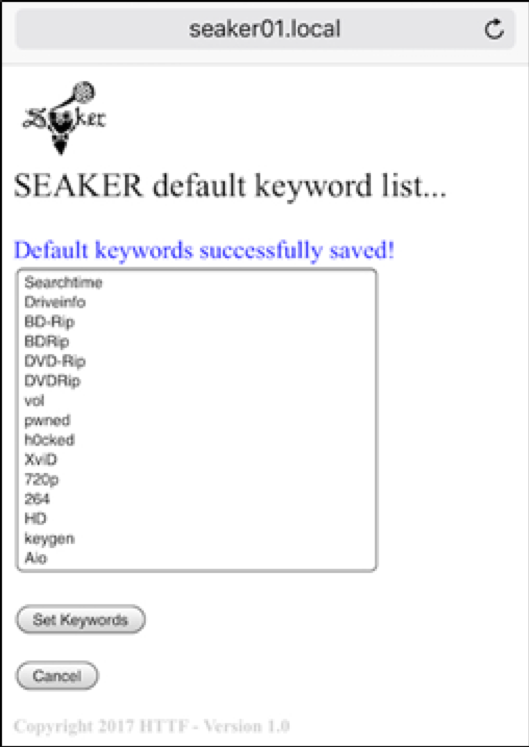
\includegraphics[width=6cm]{images/DefaultKeywords.png}
  \caption{Default Keywords page}
  \label{fig:DefaultKeywords}
  \end{center}
\end{figure}

\subsection{Process Flow}

The SEAKER device usage involves two main flows.  The first is the 
process of {\em collection}, which involves plugging it in to power
and then attaching digital media devices to it to be scanned.
The second process is {\em searching}, as discussed in a
previous section.
See Figure~\ref{fig:ProcessFlow} for details.

\begin{figure}[H]
  \begin{center}
  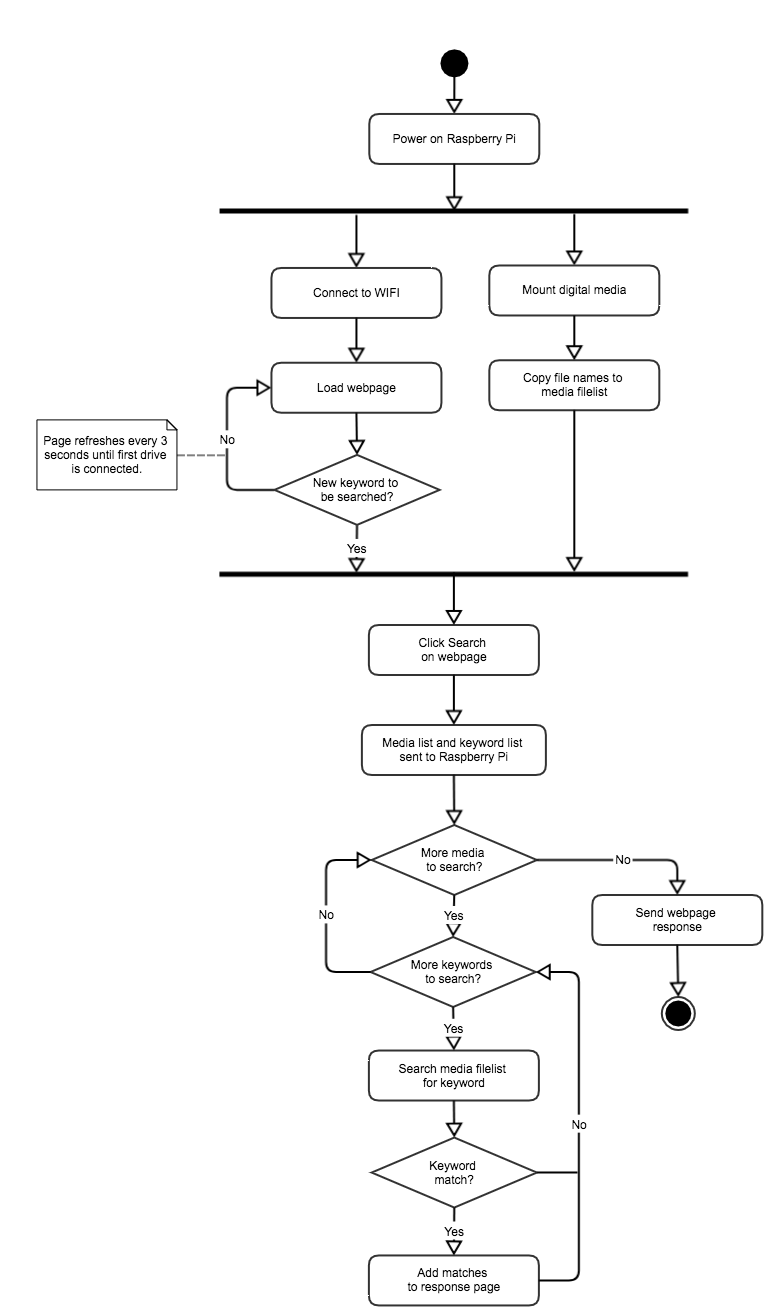
\includegraphics[width=11cm]{images/ProcessFlow.png}
  \caption{General Process Flow}
  \label{fig:ProcessFlow}
  \end{center}
\end{figure}

The process flow of SEAKER is a very simple design. After turning on
the Raspberry Pi, the two processes happen simultaneously. Immediately
when the drive(s) are connected to the Raspberry Pi, the file names
and their paths are collected and copied to a text file. Meanwhile,
the user must connect to the Raspberry Pi via WIFI on a separate
wireless-enabled device. The user must then open the SEAKER web page.
As shown in General Process Flow of Figure~\ref{fig:ProcessFlow},
the web page will refresh every 3 seconds, looking for new drives to
be connected to the Pi. The first drive will be automatically added
to the list of drives available on the webpage to be searched. All
additional drives will appear in the list when the user refreshes
the page manually.\\

All user selected drives will then go through the search process as
shown in the lower section of the General Process Flow of
Figure~\ref{fig:ProcessFlow}. Each drive will be processed one at a
time. For example, the list of files for the drive will be scanned
for any matches to the first keyword in the list. The search is done
using the regular expression tool embedded in the Raspbian Linux
operating system called {\em grep}. All files that are found to match
that keyword will be added to the output HTML. Once the entire file
list has been searched for that keyword, the process will begin again
with the next keyword in the list. This process will continue until
there are no more keywords to be searched. If multiple drives have
been selected to be searched, the same process will repeat itself
for each drive. Finally, the PHP engine will finish processing and
the HTML response page is finalized and sent back to the user's
mobile device.


\subsection{Tools Used for Development}

\subsubsection{Hardware}

TODO:\\
Raspberry Pi and power cord\\
Micro SD Card\\
Powered USB to SATA controller\\
Router or switch\\
Ethernet cable\\


\subsubsection{Programming Languages and Scripting}

TODO:\\
bash\\
c\\
HTML\\
CSS\\
PHP\\
JavaScript\\
JQuery\\
Regular Expressions via grep\\

\subsubsection {Raspbian Operating System}

TODO:\\
Raspbian Linux (a Debian distro)\\
grep\\
apt-get for os packages\\
Apache for web server\\
PHP add-on for Apache\\
Rules file for auto-mounting\\


\subsubsection{Collaboration Tools}

TODO:\\
Gliffy for charts and graphs\\
Slack for instant messaging and group chatting\\
AWS for S3 bucket\\
github for code sharing\\
Dropbox Paper for documentation collabortation\\

\subsubsection{Setup Tools}

TODO:\\
Hardwire connection to the internet\\
Macintosh: etcher, ssh, terminal, Paragon NTFS\\
Windows: Win32DiskImager, command line, putty (for ssh)\\


\section{Experimental Results}
\label{sect-experimentalResults}

\subsection{Prototype Demonstration}

TODO: in-class example at end of semester\\

\subsection{Results}

TODO: graph of latency\\

TODO: estimates of time vs data Gb\\

TODO: examples of running on Frank disks\\


\section{Conclusions and Future Work}
\label{sect-conclusionAndFutureWork}

SEAKER is currently a prototype; there are many improvements to be made, and we will discuss
some of them in this section. These improvements may be implemented by future students, or by digital
forensics professionals. We encourage anyone who implements them to share their work; the main bash
script for the SEAKER device is available on github at https://github.com/michaelsoltys/seaker.\\

First, SEAKER supports a select few filesystems. Namely, NTFS and FAT (exfat, FAT32, FAT16...).
There are likely bugs to be worked out in the supported filesystems, and there is certainly work to be
done in expanding the list of supported systems.\\

If an unsupported filesystem is in use, it may simply fail to mount, and not show up on the SEAKER
site at all. Similarly, drives from which files are currently being collected do not appear; the site displays
them only when files have been collected. Here there is opportunity for improvement; as opposed to
displaying drives for which collection is complete, SEAKER could display all drives, and a status next
to each. This status only requires three states: failed search (for unsupported systems), collection in
progress, and collection complete.\\

It can be difficult to match a hard drive to its corresponding search results. Partitions are uniquely
identified by a UUID, and some properties (capacity, for example) are displayed with the search results,
but these properties do not provide a perfect way to determine which physical device corresponds to
which mounted partition or device. Storage devices generally have a serial number of sorts, but this
serial number is not visible to SEAKER. This is a problem which requires some creativity to solve well.
SEAKER could take a picture when a drive is plugged in, and associate that picture with the search
results, for instance, but this solution requires that investigators position each storage device in front of
a camera; this approach requires a camera, and moreover it is tedious and error-prone.\\

When a search finds a hit (i.e., a matched expression or file extension), investigators may want to
view the corresponding file. Currently, this would require them to manually find and open the file. Speed
and ease of use are priorities, so it would be best if investigators could select a file in the search results
and have SEAKER fetch a copy of it for them. This function inevitably requires that the storage device
being queried is still connected—assuming that this condition is met, copying and viewing a file should
not be too complex.\\

Similarly, it would be useful if investigators could view thumbnails of images and videos in the search
results. One example of the motivation here is child pornography cases; incriminating images may have
innocuous names, but thumbnails would indicated the true content.\\

This leads to another issue: as incriminating files may be named innocuously, investigators will often
want to search simply for all images, videos, etc. SEAKER could minimize the work necessary by
allowing for preset groups of search terms, which can be created and edited by administrators. For
example, an admin could create an “images” group which causes SEAKER to include jpg, pdf, png...\\

We are very interested in a “Data Carving” option. Data carving is the identification and extraction
of files from unallocated clusters using file signatures. A file signature, also commonly referred to as a
magic number, is a constant numerical or text value used to identify a file format. The object of carving
is to identify and extract (carve) the file based on this signature information alone. We are interested in
hidden files (which are sometimes easy to locate, as for example in UNIX with {\em ls -a} command) and
deleted files, which is more tricky as the files can partially overwritten. A partially overwritten file may
still constitute valuable evidence: for example, a portion of an image can be taken as solid evidence that
the entire image was on the disk at some point. How can one establish whether a portion of an image
comes from a particular image? It seems that the only way to accomplish that is by visual inspection,
and having an investigator recognize the original image. In order to automate this process one could
attempt one of two things: build a massive database of frequently circulating (say, CP) images, and
hashing different formats of these images (.pdf, .jpg, .giff, .tiff, etc.), as well as different resolutions,
and chunks of standard sizes (say, 64Kb). This still seems like a shot in the dark. The second approach
is to define something akin to fuzzy hashes, the type of hashes that are used to recognize variants of the
same malware. This new type of fuzzy hashing would be invariant under different formats, or standard
resolutions, and chunks of an image could be identified by close proximity to the original hash. Hits
would be still confirmed visually to avoid false positives; a bigger issue would be false negatives.\\

Finally, documentation is important in any investigation. When triage reveals media which motivates
investigators to confiscate the corresponding storage device, they should document this motivation. As
such, it would aid investigators if SEAKER could generate a search report for a selected drive from
the search results screen. This report could be downloaded to the investigator’s device or saved on the
SEAKER unit for later access by an administrator. It should contain the search results along with some
circumstantial information, such as the date, the name(s) of investigator(s) requesting the report, and
their reason for confiscating the device.\\

The potential uses for the SEAKER device are great with the existing set of
functionality.  However, the future potential functionalities are even greater.\\

The general implementation and code have some limitations.  For instance,
in addition to the regular expressions, there could also be fuzzy matching, size
grouping, internet browser data, registry, swap file, and email searching, and
many others.\\

Another potential area for improvements to existing code could be a location for
entering passwords obtained from suspects.  These could be used to unlock entire
drives, zip files, PDFs, user folders, files, email, website usage, etc.  This
could also be extended to find online account passwords, especially in the case
of browsers that allow saving site-specific usernames and passwords.\\

The SCHTTF has asked for some new functionality as well.  They would like the
ability to search multiple partitions, local WIFI networks and access levels, 
thumbnails of images and videos, support newer operating systems (APFS and
HFS Plus), and extract IP addresses from known suspect configuration files and 
other locations.  These are just a few of the requests, but seemed to be at
the top of their list.\\

As well, there are many different libraries that could be included and built
into a searching algorithm.  Be aware that these will slow down the gathering
process and could be more useful if searched in stages.  Here are a few:

\begin{itemize}
  \item LibForensics http://code.google.com/p/libforensics/
  \item Volatile Memory search (Volatility: http://code.google.com/p/volatility/) and (WindowsSCOPE: http://www.windowsscope.com/)
  \item Oxygen for mobile http://www.oxygen-forensic.com/en/features
\end{itemize}

In researching this topic a lot of other potential improvement features
came to mind.  This is by no means a comprehensive list, but it is a start:

\begin{itemize}
  \item More supported media types
  \item Add AJAX (or similar technology) to give live feedback for search and collection
  \item Create RESTful API for using Raspberry Pi
  \item Clean up HTML code, use CSS
  \item Write SEAKER iPhone/iPad/Android apps to connect to Raspberry Pi and perform searches, edit keywords, etc.
  \item Use heap memory for path
  \item Better way to skip . and .. (possibly always skip first two entries?)
  \item Reduce size of file/directory listing file. This may involve changing how to grep or implementing custom grep
  \item Possibly store files in database instead of a file
  \item Implement the ability to connect to Raspberry Pi using Bluetooth instead of WIFI
  \item Customize web pages for device type
  \item Use a better wireless network adapter for better range. These adapters are inexpensive.
  \item Implement Linux setup with puppet/cfengine/salt/etc
  \item Better error messages about why drive could not be read
  \item Add a “Blinkt!” light panel to show visual status of the Raspberry Pi
  \item Check the health (SMART status) of the hard drive before scanning
  \item Add support for RAID, mSATA, SCSI hard drives (mdadm)
  \item Read directly from rawdisk to find file list to speed up collect
  \item Make SEAKER an available Raspbian/Debian package
  \item Support unicode filenames
  \item Auto-unmount the hard drive at the end of collection
  \item Support multiple partitions gracefully
  \item Search for filename matches only
  \item Search for path matches only
  \item Offer option via checkbox for searching inside compressed files
  \item Offer option via checkbox for searching inside text files
  \item Find all deleted files (foremost, ntfsundelete)
  \item Search deleted partitions and unpartitioned space
  \item Build another web page for troubleshooting/access/administration/etc
  \item Search on-media virtual hard drives (vhd, vdi, vmdk) (vmware, virtual pc, parallels, hyper-v)
  \item Search on-media hard drive images (.iso)
  \item Searching the raw drive instead of using the on-media operating system
  \item Online hard drive investigation (i.e. Cloud Forensics)
  \item Network Traffic Investigation
  \item Video segmentation and video image hashing
  \item Crime-specific searchs:
  \begin{itemize}
    \item financial crimes
    \item credit card fraud
    \item hacking
    \item bullying
    \item bloackmail
    \item espianage
    \item fraud
    \item customizable (corporate / military)
  \end{itemize}
  \item OS lockdown (raspbian)
  \item Decrypting encrypted devices (password entry location, assessment without password)
  \item Utilize forensics as a service
  \item Integrate with Microsoft's photoDNA cloud service
  \item Build an iPad app to simpler, more guided use
  \item Query Expansion - automatically searching for same query maybe other contexts
  \item Synonym Matching - automatically searching for similar words to query word
  \item Collect everything in UTC time for chronology matching
  \item Universal way of collecting hard drive hash for verification of evidence integrity
  \item Data Visualizations:
  \begin{itemize}
    \item present all data visualizations for particular drive or all hard drives
    \item graph - size vs amount of files (one hard drive, and all hard drives)
    \item graph - common details (like file type, etc) maybe clickable!
    \item graph/chart - files by date
    \item graph/chart - files by file type
    \item chart - website visits
    \item digital image hashes list (stored and compared)
    \item many others...
  \end{itemize}
  \item Improve analysis speed: skip known OS files, known applications files, etc.
  \item Investigation Gathering rollup: (possibly stored online or in a report)
  \begin{itemize}
    \item Database Schema for storing case specific data
    \item metadata
    \item Unique ``gathering ID''
    \item case number
    \item observation report
    \item crime severity
    \item potential offenses
    \item time gathered
    \item gatherer
    \item suspect list
    \item location gathered
    \item suggestions for other research
    \item which computer system it came from
    \item Set of evidence
    \item Digital Evidence item
    \item images of item
    \item unique item ID
    \item file contents
    \item ranking within set of evidence
    \item image thumbnails
    \item collection statistics
    \item etc
  \end{itemize}
  \item Find encryption Keys 
  \item Thumb strips of videos
  \item Predetermined search criteria (passwords, pw, etc)
  \item Output more file information: file owner, MAC times
  \item Sorting ability, for instance based on user or access times
  \item Ability to search by time, i.e. time=lastweek, time=5/5/18-5/15/18
  \item Internet usage timeline
  \item Auto-search / Auto-filter
  \item For drug related crimes, search... Spreadsheets, documents, databases, internet purchase strives
  \item For financial related crimes, search... Spreadsheets, databases, MSMoney, Quicken
  \item CRC of any acquired files (for later integrity comparison)
\end{itemize}

\vspace{0.4 cm}
The SEAKER project was a successful collaboration between two different institutions in the public
sector: law enforcement and academia. The former has many interesting problems to offer, but as they
are overwhelmed with cases they typically do not have the man power to do research and development.
The latter is happy to do research and development, as it enhances the educational experience of the students to be learning
in the context of applications to real life problems. It is a fortuitous and symbiotic relationship, and we
plan to embark on other such projects in the future.\\

SEAKER is also the testament to the fact that supremely useful devices, meeting the needs of
practitioners, can be constructed from relatively simple components; what is required is expertise and
enthusiasm, which in the best cases academia possesses in ample measure. RPs are a revolution in
embedded controllers, and we are just scratching the surface of their applicability. They are inexpensive,
but wield the power of the Linux OS.\\

For the students, the experience was invaluable. Perhaps the most important aspect was non-technical:
how to work well in a large team. There were eighteen students in the group; a composition of different
backgrounds, talents and strengths. We divided the task into five different but interconnected teams:
Task 1 was connecting the external devices to the RP; Task 2 was searching the contents of the
devices; Task 3 was responsible for sending the query and retrieving the results of the search to the
handheld; Task 4 was responsible for the documentation of the project (both a user set up and guide,
as well as the technical documentation of the solution); Task 5 was responsible for testing.\\

Digital forensics and academia would both benefit greatly from increased collaboration; students can
offer relatively inexpensive development in exchange for real-world experience and the opportunity to
create something which will be used. As a side effect more students would consider digital forensics
as a career, resulting in some level of alleviation of the problems mentioned in the second quote in the
introduction\cite{hitchcock2016tiered}.


\section{Appendix}
\label{sect-Appendix}

\subsection{\gls{seaker} Setup}
The following set of instructions will detail how to setup the \gls{seaker}
environment for the first time. There are three install options that
enable \gls{seaker} creators to prepare the device.  See
Table~\ref{tab:RequiredSoftware}

\begin{enumerate}
  \item {\em Router}: This option is where the \gls{rpi} and the
  secondary computer are connected directly to the same router, thus
  allowing the same local DHCP to assign the IPs of both.  The
  secondary computer is used to prepare the micro SD card and to later
  remotely and securely connect to the \gls{rpi} to complete the
  setup.
  
  \item {\em Direct Connect}: This option is where the Raspeberry Pi
  is connected directly to a monitor and keyboard to enable direct
  user input via the termnial.  The secondary computer is necessary to
  prepare the micro SD card, but not used to remotely connect to the
  \gls{rpi} to complete the set up.

  \item {\em Corporate LAN}: This option is almost identical to the
  {\em Router} option, but utilizes a corporate network instead of
  a local router to connect to the \gls{rpi}.  This option is the
  most IT intensive, since the IP address assigned to the Raspberry
  Pi is often not easily found.
\end{enumerate}

\begin{center}
  \begin{tabular}{l|l|l}\hline\hline
    {\bf Option 1}    & {\bf Option 2}         & {\bf Option 3} \\
    {\bf (Router)}    & {\bf (Direct Connect)} & {\bf (Corporate LAN)} \\\hline\hline
    \multicolumn{3}{c}{}\\
    \multicolumn{3}{c}{Hardware Required} \\
    \multicolumn{3}{c}{}\\\hline
    & & \\
    \textbullet \gls{rpi} & \textbullet \gls{rpi} & \textbullet \gls{rpi} \\
    \textbullet Mac or Windows Computer & \textbullet Mac or Windows Computer & \textbullet Mac or Windows Computer\\
    \textbullet Micro SD card & \textbullet Micro SD card & \textbullet Micro SD card\\
    \textbullet Router & \textbullet Monitor\\
    & \textbullet Keyboard\\
    & & \\\hline
    \multicolumn{3}{c}{}\\
    \multicolumn{3}{c}{Software Required} \\
    \multicolumn{3}{c}{}\\\hline
    & & \\
    \textbullet Raspian Stretch Lite & \textbullet Raspian Stretch Lite & \textbullet Raspian Stretch Lite \\
    \textbullet ssh client & \textbullet ssh client & \textbullet ssh client\\
    \textbullet Disk Imaging software & \textbullet Disk Imaging software & \textbullet Disk Imaging software\\
    \textbullet IP Scanning software & & \\
    & & \\\hline
  \end{tabular}
  \captionof{table}{\gls{seaker} set up: Required Hardware and Software}\label{tab:RequiredSoftware}
\end{center}

The following creation process is required to setup the \gls{seaker} device
to the specifications outlined in this paper.  Figure~\ref{fig:SeakerCreation} 
outlines the general process, while the specific steps are listed below.

\begin{figure}[ht]
  \begin{center}
  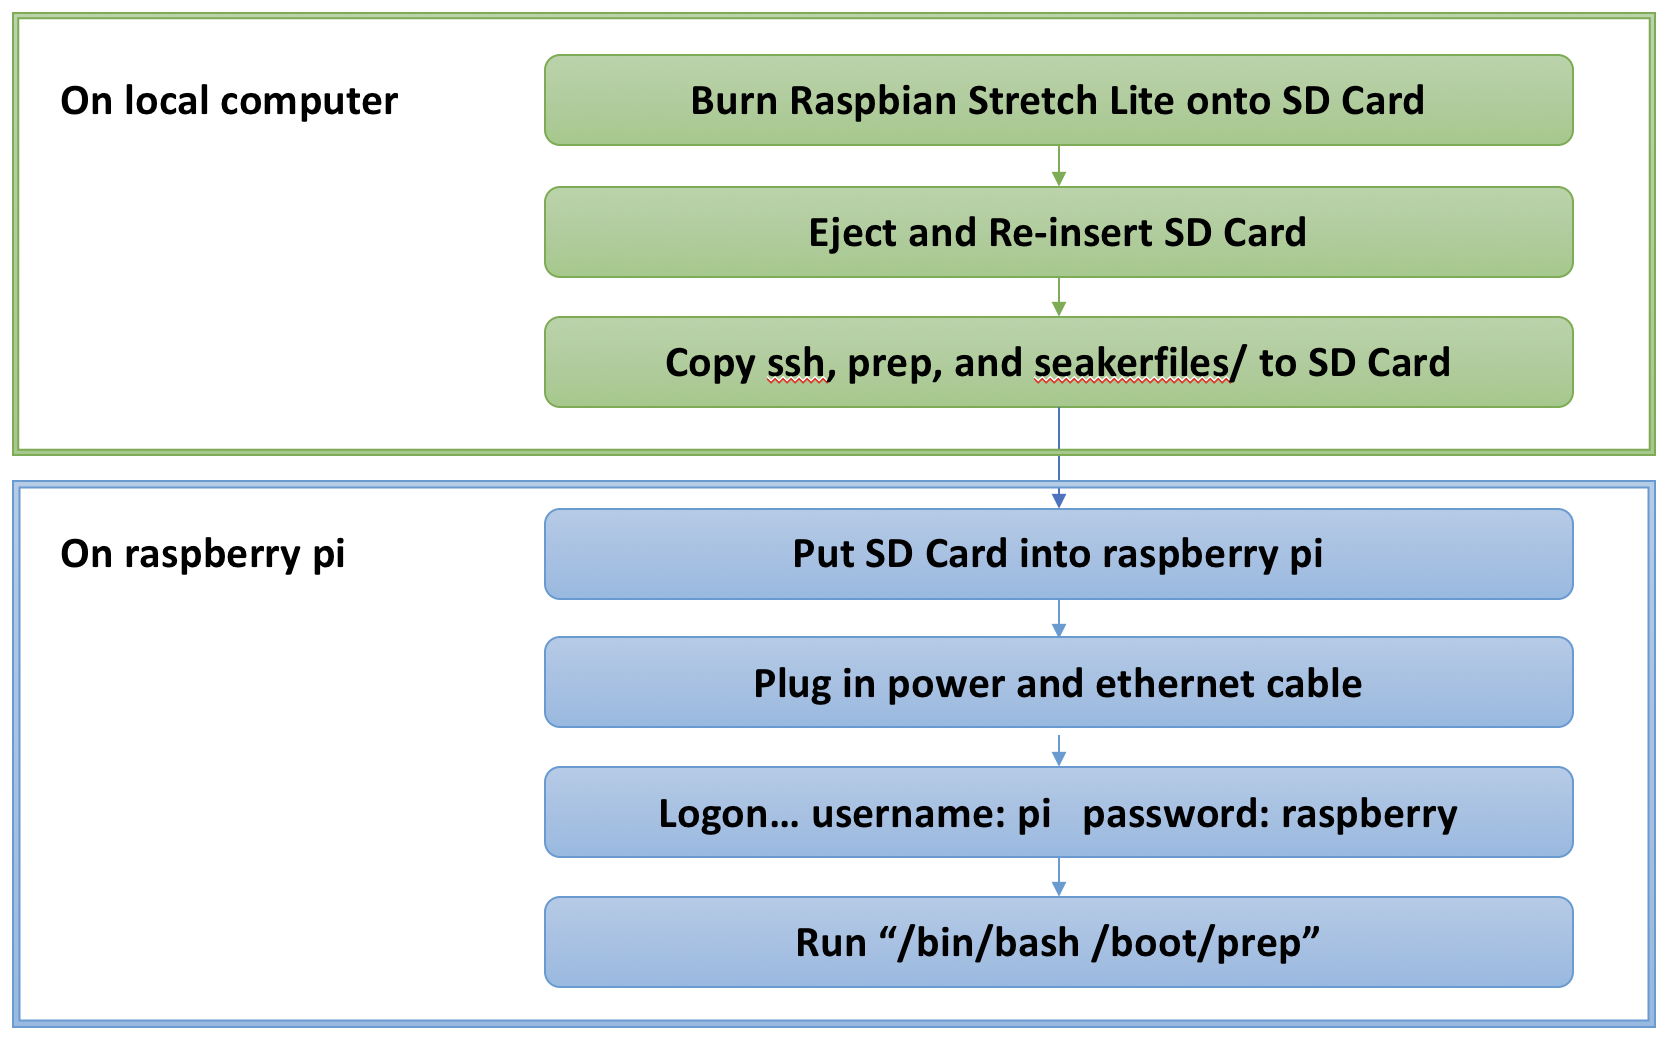
\includegraphics[width=14cm]{images/SeakerCreation.png}
  \caption{SEAKER Creation Process}\label{fig:SeakerCreation}
  \end{center}
\end{figure}

\begin{enumerate}
  \item Download the latest Raspbian Stretch Lite operating system\\
  (https://www.raspberrypi.org/downloads/raspbian/).
  Note the location where file is saved.
  \item Download the most recent copy of {\em prep.sh}, {\em ssh}, and the 
  folder called {\em seakerfiles}. These files
  contain \gls{seaker} setup and running code.
    \begin{itemize}
      \item prep.sh file location: https://s3-us-west-2.amazonaws.com/seaker/prep.sh
      \item ssh file location: https://s3-us-west-2.amazonaws.com/seaker/ssh
      \item seakerfiles location: https://s3-us-west-2.amazonaws.com/seaker/seakerfiles
    \end{itemize}
  \item Open prep.sh and edit the default configuration information
  (shown below). At minimum it is recommended to change the Raspberry
  Pi and WiFi passwords.\\

  \lstinputlisting[language=bash]{code/config.sh}

  NOTE: It is recommended to change the WIFI Name and IP Address when
  setting up multiple \gls{seaker} environments over time to ensure each
  environment has unique identifying information.\\
  \\
  For example: If setting up three \gls{seaker} environments, configuration could be:
    \begin{enumerate}
      \item Name: SEAKER01, IP Address: 192.168.101.1
      \item Name: SEAKER02, IP Address: 192.168.102.1
      \item Name: SEAKER03, IP Address: 192.168.103.1
    \end{enumerate}
  \item Insert micro SD card into computer (not the \gls{rpi}).
  An adapter will likely be required.
  \item Open disk imaging software (Etcher for Mac, or SDFormatter and 
  Win32 Disk Imager for Windows).
  Map to the Raspbian Stretch Lite file
  location, choose the micro SD card as the destination, and select to burn
  the image. (Refer to the chosen imaging software documentation for
  specific instructions on using this tool.)  Do not remove the micro SD
  card from the computer.
  \item Map to the micro SD card (Finder for Mac, File Explorer for Windows).
  Copy ssh, prep.sh, and the seakerfiles folder onto the micro SD card's
  {\em boot} partition.
  \item Remove the micro SD card from the computer.
  \item Insert the card into the \gls{rpi}.
  \item Power on the \gls{rpi} by plugging it in with the power cord.
  \item Identify the local IP Address of the \gls{rpi}:\\
  If installing with Option 1 (router):
    \begin{enumerate}
      \item Plug the \gls{rpi} into the same router being used by the
      Windows or Mac computer.
      \item Use the IP Scanning tool on the computer to find the local IP
      Address of the \gls{rpi}. The Manufacturer should be ‘Raspberry
      Pi Foundation’.
    \end{enumerate}
  If installing with Option 2 (Direct Connect):
    \begin{enumerate}
      \item Connect the monitor and keyboard to the \gls{rpi}.
      \item Login using the default username (pi) and password (raspberry).
      \item Enter the following command to retrieve the local IP Address:\\
      \begin{verbatim}
        ifconfig eth0
      \end{verbatim}
    \end{enumerate}
  If installing with Option 3 (Corporate Network):
    \begin{enumerate}
      \item The MAC Address of the \gls{rpi} is required. This can be
      located on the original \gls{rpi} box.
      \item For Windows systems, open a command prompt and enter the command
      below. Replace the ``c8:26:3b:d2:63:d5'' sequence with the MAC Address
      of the \gls{rpi} being configured.  Use the following command:
      \begin{verbatim}
        arp -a | findstr "c8:26:3b:d2:63:d5"
      \end{verbatim}
      \item For Unix or Linux systems such as Apple or Ubuntu, open a terminal
      window and enter the command below. Replace the ``c8:26:3b:d2:63:d5''
      sequence with the MAC Address of the \gls{rpi} being configured.
      Use the following command:
      \begin{verbatim}
        arp -a | grep "c8:26:3b:d2:63:d5"
      \end{verbatim}
    \end{enumerate}
  \item If installing with Option 1 or 3:
    \begin{itemize}
      \item SSH into the \gls{rpi} from the laptop or desktop computer.
      \begin{itemize}
        \item If using a client such as Putty, enter the local IP address
        of the \gls{rpi}, choose SSH and connect. Click \verb|OK| or
        \verb|Yes| on the security warning.
        \item If using a command line utility such as Bash enter the
        following at the prompt:
        \begin{verbatim}
          ssh pi@<ip_address> -l pi
        \end{verbatim}
        \item Login using the default username (\verb|pi|) and password
        (\verb|raspberry|).
      \end{itemize}
    \end{itemize}
  \item Run the preparation script by typing the following on the command line:
  \begin{verbatim}
    /bin/bash /boot/prep.sh
  \end{verbatim}
  \item Wait for the \gls{rpi} to finish running the script and
  rebooting. The \gls{rpi} should now be configured as a \gls{seaker}
  and be up and running.
\end{enumerate}

\newpage
\subsection{\gls{seaker} Usage}

After collecting all the media devices at the scene, the investigator
will triage them with \gls{seaker}.  Each step of the process is broken
down and discussed in detail below.\\

(1)~Connect the RP to the power and wait for about a minute
to let it finish booting up.
Connect to the RP's Wireless Access Point (WiFi network). Depending
on the setup, the WiFi's SSID will be ``SEAKER01'' or ``SEAKER02''
etc.  See Figure~\ref{fig:screen-1}. Note that \gls{seaker}'s Wireless Access
Point is password
protected and matches the one specified in the prep.sh script file.\\

\begin{figure}[ht]
  \begin{center}
  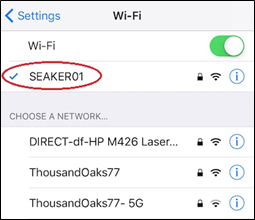
\includegraphics[width=6cm]{images/seaker-hh-screen-1.jpg}
  \caption{iPhone WIFI connection to the \gls{seaker}.}\label{fig:screen-1}
  \end{center}
\end{figure}

(2)~At the same time the investigator may connect all the media
devices to the RP. This may be done concurrently with the previous
step. Note that in order to examine a digital media it will need to be
removed from the
computer, and connected to the RP; this may be done through a
write-blocker interface but it is not necessary.\\

(3)~Once connected to the \gls{seaker}'s Wireless Access Point,
the investigator will open any
web browser on their connected device and direct it to go to
\verb|http://seaker01.local|. Access is allowed
through a web browser, as this is the most universal way to connect
on any device (iPhone, iPad, Android, laptop, etc.).  These
devices and many more can connect to a Wireless Access Point
and open a browser.  Once the browser establishes the
connection, the user will see Figure~\ref{fig:screen-2}. Note that the
keywords (or regular expression patterns) present in the ``Type in
Search Terms:'' can be pre-loaded before arriving at the scene, or
changed/updated at the scene.\\

\begin{figure}[H]
  \begin{center}
  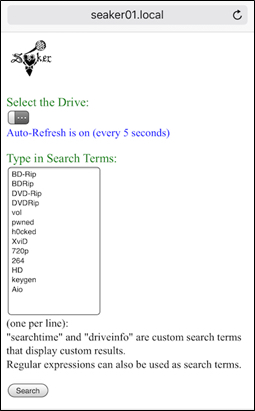
\includegraphics[width=6cm]{images/seaker-hh-screen-2.jpg}
  \caption{Using a browser to connect to {\tt http://seaker01.local}}
  \label{fig:screen-2}
  \end{center}
\end{figure}

The regular expression can be given using the syntax of the
\verb|grep| utility. For example, if we want to find occurrences of
either `two' or `too', we use \verb|t[wo]o|; if we want to find every
word that start with capital letters, we use \verb|^[A-Z]|; if we want
to find words where number~9 is the last character of the line, we use
\verb|9$|. There are a vast number of possibilities; we can also
replace \verb|grep| with \verb|egrep| that has an even richer syntax.\\

(4)~Once any storage media devices that are found at a search warrant scene
are connected to the RP, the investigator will typically wait for a
few minutes (with some times up to 10 minutes for 1Tb disks with
millions of files) for the file list to be built. Searches can then
be carried out very quickly; essentially, \verb|grep| browses the file
list, line by line, outputting those lines that conform to at least
one pattern specified in the ``Type in Search Terms:'' window. Once
this finishes, the investigator will have the results presented as in
Figure~\ref{fig:screen-3}.

\begin{figure}[H]
  \begin{center}
  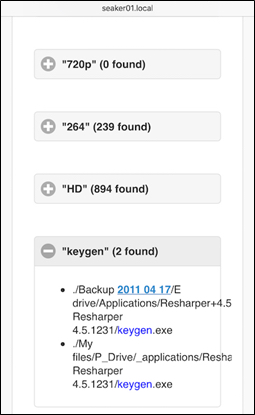
\includegraphics[width=6cm]{images/seaker-hh-screen-3.jpg}
  \caption{The results of the search of a particular device.}
  \label{fig:screen-3}
  \end{center}
\end{figure}

The filenames themselves can be incriminating evidence, such as in
Child Pornography (CP) cases, where the material has a commonly used
naming convention, e.g., ``lolita'' which can be found with the grep
pattern \verb|.*lolita.*| (`\verb|.*|' means the
following: `\verb|.|' (period)  matches any single character of any
value, except
a newline, and `\verb|*|' (asterisk) matches zero or more of the
preceding character or expression) or simply \verb|lolita|.
This can be used by the
investigators to question the suspects.  The questioning usually
takes place at the same time as the forensic examiners triage the
evidence, and one of the requirements of \gls{seaker} was to be fast so that
investigators can start getting intelligence quickly from the initial
processing of the scene.\\

(5)~The user process flow is documented in the following
figure~\ref{fig:user_process_flow}.

\begin{figure}[ht]
  \begin{center}
  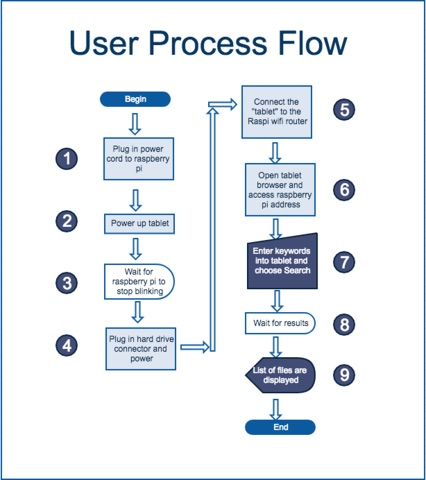
\includegraphics[width=10cm]{images/user_process_flow.jpg}
  \caption{The functionality of \gls{seaker} from the user perspective.}
  \label{fig:user_process_flow}
  \end{center}
\end{figure}

\newpage
\subsection{Code}
\subsubsection{Directory and Filename Collection Code (in C)}
\lstinputlisting[language=bash]{code/collect_files.c}

\newpage
\subsection{Results of Testing}
\subsubsection{Collection Timing}

For testing purposes, ls was optimized to utilize as few time-consuming
options as possible, including the {\em -f} option that prevents sorting
and {\em -A} for skipping current and parent directories (. and ..)
in the results.
Here are the actual functions used:

\vspace{0.1 cm}
\begin{verbatim}
  sudo sh -c 'cd /mnt/usb && time ls -ARf1 > ~/ls_time.txt'
  sudo sh -c 'cd /mnt/usb && time find / -print > ~/find_time.txt'
  sudo sh -c 'cd /mnt/usb && time ~/collect > ~/collect_time.txt'
\end{verbatim}
\vspace{0.1 cm}

Testing results for the custom collection code vs. operating system file
and directory listing applications:

\begin{center}
  \tiny
    \begin{tabular}{|l|r|r|r|r|r|l|}
    \hline
    \textbf{}                        & \multicolumn{1}{l|}{\textbf{SSD}} & \multicolumn{1}{l|}{\textbf{SSD}} & \multicolumn{1}{l|}{\textbf{\begin{tabular}[c]{@{}l@{}}WD 2.5'\\ SATA HDD\end{tabular}}} & \multicolumn{1}{l|}{\textbf{\begin{tabular}[c]{@{}l@{}}iOmega 3.5'\\ IDE HDD\end{tabular}}} & \multicolumn{1}{l|}{\textbf{\begin{tabular}[c]{@{}l@{}}Samsung 3.5'\\ SATA HDD\end{tabular}}} & \textbf{}                          \\ \hline
    \textbf{Size GB}                 & 500                               & 500                               & 500                                                                                      & 1000                                                                                        & 1000                                                                                          &                                    \\ \hline
    \textbf{Consumed GB}             & 94.22                             & 239.83                            & 456                                                                                      & 474.2                                                                                       & 316.6                                                                                         &                                    \\ \hline
    \textbf{\% Consumed}             & 18.84\%                           & 47.97\%                           & 91.20\%                                                                                  & 47.42\%                                                                                     & 31.66\%                                                                                       &                                    \\ \hline
    \textbf{\# files}                & 1,244,699                         & 1,561,132                         & 14,487                                                                                   & 216,356                                                                                     & 21,556                                                                                        &                                    \\ \hline
    \textbf{\# directories}          & 254,473                           & 317,876                           & 145                                                                                      & 10,603                                                                                      & 2,222                                                                                         &                                    \\ \hline
    \textbf{ls t1}                   & 62.142                            & 112.627                           & 0.942                                                                                    & 8.398                                                                                       & 1.400                                                                                         &                                    \\ \hline
    \textbf{ls t2}                   & 62.025                            & 116.978                           & 0.899                                                                                    & 8.252                                                                                       & 1.375                                                                                         &                                    \\ \hline
    \textbf{ls t3}                   & 68.376                            & 115.833                           & 0.903                                                                                    & 8.229                                                                                       & 1.324                                                                                         &                                    \\ \hline
    \textbf{ls ave time (secs)}      & \textbf{64.181}                   & \textbf{115.146}                  & \textbf{0.915}                                                                           & \textbf{8.293}                                                                              & \textbf{1.366}                                                                                & \textbf{}                          \\ \hline
    \textbf{find t1}                 & 43.914                            & 90.693                            & 1.004                                                                                    & 9.090                                                                                       & 1.733                                                                                         &                                    \\ \hline
    \textbf{find t2}                 & 44.958                            & 97.619                            & 1.014                                                                                    & 8.315                                                                                       & 1.667                                                                                         &                                    \\ \hline
    \textbf{find t2}                 & 43.214                            & 96.499                            & 1.015                                                                                    & 8.347                                                                                       & 1.672                                                                                         &                                    \\ \hline
    \textbf{find ave time (secs)}    & \textbf{44.029}                   & \textbf{94.937}                   & \textbf{1.011}                                                                           & \textbf{8.584}                                                                              & \textbf{1.691}                                                                                & \textbf{}                          \\ \hline
    \textbf{col t1}                  & 20.893                            & 68.270                            & 0.834                                                                                    & 7.541                                                                                       & 1.281                                                                                         &                                    \\ \hline
    \textbf{col t2}                  & 18.103                            & 82.091                            & 0.832                                                                                    & 7.548                                                                                       & 1.260                                                                                         &                                    \\ \hline
    \textbf{col t3}                  & 19.381                            & 84.823                            & 0.804                                                                                    & 7.531                                                                                       & 1.248                                                                                         &                                    \\ \hline
    \textbf{collect ave time (secs)} & \textbf{19.459}                   & \textbf{78.395}                   & \textbf{0.823}                                                                           & \textbf{7.540}                                                                              & \textbf{1.263}                                                                                & \textbf{Average:}                  \\ \hline
    \textbf{\% faster than ls}       & 70\%                              & 32\%                              & 10\%                                                                                     & 9\%                                                                                         & 8\%                                                                                           & \multicolumn{1}{r|}{\textbf{26\%}} \\ \hline
    \textbf{\% faster than find}     & 56\%                              & 17\%                              & 19\%                                                                                     & 12\%                                                                                        & 25\%                                                                                          & \multicolumn{1}{r|}{\textbf{26\%}} \\ \hline
    \end{tabular}
  \captionof{table}{Collection Algorithm Timing Data}\label{tab:CollectionAlgorithmData}
\end{center}

TODO: add more result data\\

\newpage
\bibliographystyle{plain}
\bibliography{references}








































\newpage

\section{STOP HERE - Abstract}
\label{sect-abstract}

Goals:
\begin{itemize}
  \item preserve and protect evidenciary integrity
  \item reduce evidence gathering and triage analysis time
  \item prevent adding more to backlog than necessary by preventing over-confiscation
  \item reduce need for on-scene Digital Forensic Ssientists
  \item reduce backlog of digital evidence for tackling backlog
\end{itemize}

\gls{seaker} tradeoffs: Precision (only relevant files) vs Recall (all relevant files)
- level of recall required at triage stage can be sacraficed\\

Introduce online storage system for digital forensic metadata format to enhance sharing capabilities across
jurisdiction boundaries and prevent sharing complexities

\section{Meetings with Frank}
\label{sect-frank}
\vspace{0.5 cm}
\subsection{May 18th, 2018}

My meeting with Frank Lyu, a civilian working for the Ventura County Sherriff's department, on loan to
the Southern California High Tech Task Force (SCHTTF) went well.  The SCHTTF is an 8 person team made up of
four civilians and four deputies, all reporting directly to the Ventura County District Attorney's office.
We met for lunch and I was able to ask him questions about the environment he works in as well as touch on
ranking the high value items that this SEAKER project could provide.\\

First, we talked about his work environment.  He has several responsibilities working for SCHTTF.  The first
and foremost is his caseload, which consists of examining digital evidence using forensic techniques in his
lab that result in a report to the District Attorney's office.  His other responsibilites include assisting
the District Attorney and staff with evaluating defense evidence reports, studying digital forensic 
technologies (for when he has to explain things to juries), helping other agencies identify and catalog
evidence that they are not familiar with, helping serve warrants on critical cases, and helping to retrieve
lost digital materials for other law enforcement agencies.

He explained that following the processes and procedures is by far the most important aspect of his job.  The
evidence handling, storage, and evaluation are critical to whether a case succeeds or is dismissed. Frank
began to describe the intake process, which involves the evidence, the agency report, and the search warrant
that will be used to search and evaluation the materials.  We did not go into further detail.

Items he looks for during an on-site warrant are: user accounts, previewing the materials (especially in
cases involving CP), and checking for the existence of Peer-to-Peer sharing utilities.  In addition, he 
strives to collect the following networking information: publically broadcast SSIDs, each SSID's level of
encryption, how many devices are connected to the router, and the external IP address for the router.

Value of SEAKER in the field: Filename search utilizing regular expression, the networking information 
specified in the last paragraph, producing a report, making an ios app instead of using a webpage, links
for the files found, and clickable thumbnails.

Value of SEAKER in the lab: Filename search utilizing regular expression and SEAKER hashes of images.  He
also mentioned a Microsoft tool called PhotoDNA that they currently use to find naked humans.

I asked about obtaining all of the statistics related to ingestion or evidence, caseload, pace at which
evidence can be evaluated, etc.  Frank's answer was that Adam could probably provide that information
without lab access, but that Michael should be asked to talk to Adam.

Finally, Frank mentioned that sometimes in financial cases, he is asked to search computers at business
offices, and the ability to search for specific filenames is very important there.

\newpage
\section{Background}
\label{sect-background}

\subsection{Introduction to Terms}
\vspace{0.5 cm}
\subsubsection{DEFR and DES Investigation Roles}
\vspace{0.5 cm}
DEFR is Digital Evidence First Responder\\

DES is Digital Evidence Specialiat\\

\subsubsection{Digital vs. Physical Evidence}
\vspace{0.5 cm}
I believe there should be a section here that examines (or at least introduces) the differences and similarities
between regular physical (non-digital) evidence and digital evidence.  Including in the analysis is the metaphore of
how physical evidence is handled (bags, DNA, fingerprints) and how that directly relates to the digital evidence
model.  Contamination must be avoided.\\

\subsubsection{Reactive vs. Proactive Digital Forensic Investigation Processes}
\vspace{0.5 cm}
\textit{Reactive} digital forensic investigation processes are utilized after an offense has been committed to help
identify the charges and suspects.  This is the most common process for digital forensics.  The \textit{proactive}
digital forensic investigation processes are to attempt to detect before or during an active offense is committed.
This is not a job for a typical law enforcement investigator.\\

This research is based on the reactive digital forensic investigation process in the hopes of reducing the digital
forensic lab backlogs across the country and world in two ways.  The first way is to reduce the amount of digital
evidence acquired for the digital forensics lab by enabling efficient and effective on-site triage to occur by
utitizing the commonality of digital evidence collection and analysis into a single step.  The SEAKER digital
evidence triage tool enables an initial collection of information and subsequent searches by any number of local,
on-scene investigators.  These investigators do not need extensive training in digital forensics to utilize it.\\

The second way is to help reduce the existing backlog by enabling a faster, more streamlined approach to initial
potential evidence gathering and reporting.  This approach utilizes the SEAKER digital evidence trial tool to 
perform an initial acquisition and analysis on every exiting case to provide a ``first-look'' at the information.  This
also enables a searching mechanism within a few minutes of plugging in digital evidence media to enable digital 
forensic investigators a quick review of materials.  The process will help with prioritization of evidence, a basic
analysis and potentially initial evidence in the form of a report that can be provided to investigators and
prosecutors.\\

\section{SEAKER Creation}
\label{sect-Creation}

\section{Analysis}
\label{sect-analysis}

\subsection{Process for gathering digital evidence}

First of all, never boot a computer.  That will alter the original state of the hard drive due to the operating
system being loaded.  This may alter the data available for collection and render the digital media ``spoiled'' and
therefore unusable ad evidence in a case.\\

The main point here is to preserve evidentiary integrity and protect against spoilage.\\

Specific training is required to be able to handle digital evidence properly.  What do digital evidence collectors
already have to go through in terms of training?\\

\newpage
\section{Keywords and glossary}
\begin{itemize}
  \item Contraband files
  \item stages: preprocessing, storage, analysis, reporting
  \item stages: gather (document, catalog), triage (analyze, live review, automated review, artifact storage,
  meet threshold?), results (present, graphs, search)
  \item Chain of Custody for digital evidence
  \item Forensic integrity of digital evidence
  \item artifacts = pieces of digital evidence that are of importance to the case
  \item enhanced previewing - better than triage (full drive)
  \item Indecent Image of Children
  \item Image Hash Databases - dbs of digital forensic labs with image hashes
  \item obviate the need for write blockers
  \item early look intelligence gathering
  \item Immediate feedback loop for onsite investigators
  \item ``Suspect's dwelling''
  \item securing a conviction of the offender
  \item protecting future victims
  \item browser artifacts
  \item onsite == in situ
  \item adhere to proven forensic principles
\end{itemize}

\newpage
\section{Graphs, Images, Figures, and tables}
\begin{itemize}
  \item figure - field triage flowchart
  \item figure - each stage field triage flowchart
  \item figure - Image analysis and hash creation flowchart
  \item graph - aquisition time vs full
  \item graph - investigation time vs full
  \item graph - analysis time vs full
  \item graph - total time from initial plug-in to decision to be evidence (threshold)
  \item graph - current backlock in ventura county
  \item figure - DFT vs TCU (Hitchcock\cite{hitchcock2016tiered})
  \item graph - collection time vs number and size of files
  \item figure - see figures in Computer Forensic Field Triage Process model (Rogers)
  \item graph - speed of collecting evidence from same drive based on microSD card used

\end{itemize}

\end{document}

